% Options for packages loaded elsewhere
\PassOptionsToPackage{unicode}{hyperref}
\PassOptionsToPackage{hyphens}{url}
%
\documentclass[
]{book}
\title{The Gatekeeper's Notebook}
\author{Kadek Adit Wiryadana}
\date{2022-02-15}

\usepackage{amsmath,amssymb}
\usepackage{lmodern}
\usepackage{iftex}
\ifPDFTeX
  \usepackage[T1]{fontenc}
  \usepackage[utf8]{inputenc}
  \usepackage{textcomp} % provide euro and other symbols
\else % if luatex or xetex
  \usepackage{unicode-math}
  \defaultfontfeatures{Scale=MatchLowercase}
  \defaultfontfeatures[\rmfamily]{Ligatures=TeX,Scale=1}
\fi
% Use upquote if available, for straight quotes in verbatim environments
\IfFileExists{upquote.sty}{\usepackage{upquote}}{}
\IfFileExists{microtype.sty}{% use microtype if available
  \usepackage[]{microtype}
  \UseMicrotypeSet[protrusion]{basicmath} % disable protrusion for tt fonts
}{}
\makeatletter
\@ifundefined{KOMAClassName}{% if non-KOMA class
  \IfFileExists{parskip.sty}{%
    \usepackage{parskip}
  }{% else
    \setlength{\parindent}{0pt}
    \setlength{\parskip}{6pt plus 2pt minus 1pt}}
}{% if KOMA class
  \KOMAoptions{parskip=half}}
\makeatother
\usepackage{xcolor}
\IfFileExists{xurl.sty}{\usepackage{xurl}}{} % add URL line breaks if available
\IfFileExists{bookmark.sty}{\usepackage{bookmark}}{\usepackage{hyperref}}
\hypersetup{
  pdftitle={The Gatekeeper's Notebook},
  pdfauthor={Kadek Adit Wiryadana},
  hidelinks,
  pdfcreator={LaTeX via pandoc}}
\urlstyle{same} % disable monospaced font for URLs
\usepackage{longtable,booktabs,array}
\usepackage{calc} % for calculating minipage widths
% Correct order of tables after \paragraph or \subparagraph
\usepackage{etoolbox}
\makeatletter
\patchcmd\longtable{\par}{\if@noskipsec\mbox{}\fi\par}{}{}
\makeatother
% Allow footnotes in longtable head/foot
\IfFileExists{footnotehyper.sty}{\usepackage{footnotehyper}}{\usepackage{footnote}}
\makesavenoteenv{longtable}
\usepackage{graphicx}
\makeatletter
\def\maxwidth{\ifdim\Gin@nat@width>\linewidth\linewidth\else\Gin@nat@width\fi}
\def\maxheight{\ifdim\Gin@nat@height>\textheight\textheight\else\Gin@nat@height\fi}
\makeatother
% Scale images if necessary, so that they will not overflow the page
% margins by default, and it is still possible to overwrite the defaults
% using explicit options in \includegraphics[width, height, ...]{}
\setkeys{Gin}{width=\maxwidth,height=\maxheight,keepaspectratio}
% Set default figure placement to htbp
\makeatletter
\def\fps@figure{htbp}
\makeatother
\setlength{\emergencystretch}{3em} % prevent overfull lines
\providecommand{\tightlist}{%
  \setlength{\itemsep}{0pt}\setlength{\parskip}{0pt}}
\setcounter{secnumdepth}{5}
\newlength{\cslhangindent}
\setlength{\cslhangindent}{1.5em}
\newlength{\csllabelwidth}
\setlength{\csllabelwidth}{3em}
\newlength{\cslentryspacingunit} % times entry-spacing
\setlength{\cslentryspacingunit}{\parskip}
\newenvironment{CSLReferences}[2] % #1 hanging-ident, #2 entry spacing
 {% don't indent paragraphs
  \setlength{\parindent}{0pt}
  % turn on hanging indent if param 1 is 1
  \ifodd #1
  \let\oldpar\par
  \def\par{\hangindent=\cslhangindent\oldpar}
  \fi
  % set entry spacing
  \setlength{\parskip}{#2\cslentryspacingunit}
 }%
 {}
\usepackage{calc}
\newcommand{\CSLBlock}[1]{#1\hfill\break}
\newcommand{\CSLLeftMargin}[1]{\parbox[t]{\csllabelwidth}{#1}}
\newcommand{\CSLRightInline}[1]{\parbox[t]{\linewidth - \csllabelwidth}{#1}\break}
\newcommand{\CSLIndent}[1]{\hspace{\cslhangindent}#1}
\ifLuaTeX
  \usepackage{selnolig}  % disable illegal ligatures
\fi

\begin{document}
\maketitle

{
\setcounter{tocdepth}{1}
\tableofcontents
}
\renewcommand\chaptername{BAB}

\addto{\captionsenglish}{\renewcommand*{\contentsname}{Table of contents}}

\hypertarget{sepatah-kata}{%
\chapter{Sepatah Kata}\label{sepatah-kata}}

Dokter jaga Unit Gawat Darurat merupakan penjaga pintu gerbang utama di fasilitas pelayanan kesehatan tingkat lanjut. Pada pelaksanaanya sering kali disertai ketiadaan panduan awal dan ketidaklengkapan SOP sehingga hanya mengandalkan ilmu dengar yang ditransfer antar telinga. Tidak jarang akan terjadi kekeliruan sehingga menghambat jalannya pelayanan kesehatan. Buku ini khusus disusun untuk memberikan panduan umum dokter jaga berdasarkan pengalaman penulis beserta hasil diskusi dengan teman sejawat dan konsultasi dengan dokter Spesialis dan Manajemen. Penulis berharap buku ini dapat membantu dokter jaga baru dalam menyesuaikan diri terhadap lingkungan dan alur kerja di Rumah Sakit kami.

\hypertarget{panduan}{%
\section{Panduan}\label{panduan}}

Buku ini hanya berisikan panduan umum. Buku tidak disusun dengan tujuan menjadi panduan komprehensif ataupun Cheatsheet. Tetap sesuaikan dengan kondisi dan selalu dengarkan kata hati.

Buku disusun atas dasar niat penulis untuk menyebarluaskan informasi antar dokter umum. Penyusunan buku dilakukan pada waktu luang penulis tanpa ada motivasi keuntungan finansial ataupun sponsor. Penulis mohon maaf dan permakluman jika terdapat kesalahan ketik atau kekeliruan isi.

\hypertarget{narahubung}{%
\section{Narahubung}\label{narahubung}}

Buku disusun oleh dr. Kadek Adit Wiryadana. Pertanyaan dan saran dapat disampaikan secara lisan atau tulisan melalui email ke \href{mailto:ka.wiryadana@gmail.com}{\nolinkurl{ka.wiryadana@gmail.com}} atau \href{mailto:wiryadana@wiryadana.org}{\nolinkurl{wiryadana@wiryadana.org}}.

\hypertarget{akses-dan-panduan-penggunaan-buku}{%
\section{Akses dan Panduan Penggunaan Buku}\label{akses-dan-panduan-penggunaan-buku}}

Buku dapat diakses secara elektronik atau cetak. Pada buku elektronik terdapat fasilitas navigasi. Panel sisi kiri merupakan Bab Buku (Daftar isi) dan pada panel sisi kanan merupakan daftar subbab dan hierarkinya pada Bab yang dipilih. Gunakan panel sisi kiri dan kanan untuk mempermudah navigasi isi buku. Terdapat fasilitas ``search'' pada panel kiri bagian atas. Akurasi ``Search'' dapat mencapai tingkat Bab, subbab dan kata/kalimat di seluruh buku. Pada buku versi PDF, terdapat ``bookmark'' yang telah disesuaikan dengan Bab buku.

\begin{itemize}
\tightlist
\item
  Buku versi elektronik untuk web dapat diakses pada tautan berikut : \url{https://wiryadana.github.io/Gateskeeper_Notebook/}
\end{itemize}

\begin{center}
\includegraphics{index_files/figure-latex/qrcode-1} \end{center}

\begin{itemize}
\tightlist
\item
  Buku versi cetak dapat dilihat di UGD. Versi PDF buku cetak dapat diunduh di : \url{https://github.com/wiryadana/Gateskeeper_Notebook/raw/master/docs/Pocket_book.pdf}
\end{itemize}

\begin{center}
\includegraphics{index_files/figure-latex/qrcode_2-1} \end{center}

\hypertarget{ucapan-terimakasih}{%
\section{Ucapan Terimakasih}\label{ucapan-terimakasih}}

Buku ini, baik versi elektronik atau cetak, terwujud seluruhnya berkat teknologi informasi bebas dan ``open source.'' Buku dibuat dengan Rmarkdown package\footnote{\emph{Rmarkdown: Dynamic Documents for r}, 2021, \url{https://CRAN.R-project.org/package=rmarkdown}.} yang digabungkan dengan program Bookdown\footnote{Yihui Xie, \emph{Bookdown: Authoring Books and Technical Documents with r Markdown}, 2021, \url{https://CRAN.R-project.org/package=bookdown}.} dan Knitr package.\footnote{Yihui Xie, \emph{Knitr: A General-Purpose Package for Dynamic Report Generation in r}, 2021, \url{https://yihui.org/knitr/}.} QR code dibuat dengan qrcode package.\footnote{\emph{Qrcode: Generate QRcodes with r. Version 0.1.4}, 2021, \url{https://doi.org/10.5281/zenodo.5040088}.} Semua program tersebut berjalan diatas bahasa pemrograman statistik R v4.1.2\footnote{R Core Team, \emph{R: A Language and Environment for Statistical Computing} (Vienna, Austria: R Foundation for Statistical Computing, 2021), \url{https://www.R-project.org/}.} pada Rstudio server\footnote{Rstudio, {``{RStudio}: {Integrated} {Development} for {R}''} (Boston: Rstudio PBC, 2021), \url{http://www.rstudio.com/}.} dan sistem operasi GNU/Linux Ubuntu Server (versi 21.04).\footnote{Canonical, {``Ubuntu {Server}''} (London, 2021), \url{https://wiki.ubuntu.com/FocalFossa/ReleaseNotes?_ga=2.202901329.1166669392.1642903327-1244252401.1642903327}.} Semua ``Source Code'' serta versi elektronik buku dapat diakses pada repository Github.

\hypertarget{smf-dokter-umum}{%
\chapter{SMF Dokter Umum}\label{smf-dokter-umum}}

Para Dokter Umum di RS bernaung dibawah satuan medik fungsional (SMF) tersendiri yaitu SMF Dokter Umum

\hypertarget{struktur-dan-anggota-smf-dokter-umum}{%
\section{Struktur dan Anggota SMF Dokter Umum}\label{struktur-dan-anggota-smf-dokter-umum}}

\hypertarget{koordinator-desember-2021---agustus-2022}{%
\subsection{Koordinator (Desember 2021 - Agustus 2022)}\label{koordinator-desember-2021---agustus-2022}}

\begin{itemize}
\tightlist
\item
  dr. Kadek Adit Wiryadana
\end{itemize}

\hypertarget{anggota}{%
\subsection{Anggota}\label{anggota}}

\begin{itemize}
\tightlist
\item
  dr. Iska Novi Udayani (\textbf{Fulltime})
\item
  dr. Ngurah Agung Reza Satria Nugraha Putra (\textbf{Fulltime})
\item
  dr. Agustin J Nanda De niro (\textbf{Fulltime})
\item
  dr. Made Vidyasti Laksita Wijaya (\textbf{Fulltime})
\item
  dr. I Gusti Agung Anggia Noverina (\textbf{Hemodialisis})
\item
  dr. Putu Eka Putra Adnyana
\item
  dr. Dwi Meviyanti
\item
  dr. M. Azman Pasha
\item
  dr. Gede Dewagama M
\item
  dr. Michael Oliver Wijaya
\item
  dr. Kadek Dwi Wira Sanjaya
\item
  dr. Gracia Dewitacita Tanaya
\end{itemize}

\hypertarget{peraturan-kerja}{%
\chapter{Peraturan Kerja}\label{peraturan-kerja}}

Hal-hal yang perlu dipatuhi saat bekerja

\hypertarget{jam-kerja}{%
\section{Jam Kerja}\label{jam-kerja}}

Jam kerja dibagi menjadi tiga shift.

\begin{itemize}
\item
  Pagi (08.00 - 14.00 Wita)
\item
  Sore (14.00 - 20.00 Wita)
\item
  Malam (20.00 - 08.00 Wita)
\end{itemize}

\hypertarget{poin-kerja}{%
\section{Poin Kerja}\label{poin-kerja}}

\hypertarget{khusus-fultime}{%
\subsection*{khusus Fultime}\label{khusus-fultime}}
\addcontentsline{toc}{subsection}{khusus Fultime}

Sesuai dengan kontrak, jaga dihitung dengan poin dengan rincian:

\begin{itemize}
\item
  Jaga Pagi \textasciitilde{} 1 poin
\item
  Jaga Sore \textasciitilde{} 1 Poin
\item
  Jaga Malam \textasciitilde{} 2 Poin
\end{itemize}

Dokter kontrak dalam sebulan minimal mendapatkan 24 poin.

\hypertarget{poin-kerja-part-time}{%
\subsection*{Poin Kerja Part-time}\label{poin-kerja-part-time}}
\addcontentsline{toc}{subsection}{Poin Kerja Part-time}

Dokter Part-time diberikan kesempatan untuk memilih waktu jaga, jika ada shift dimana tidak bisa diisi oleh dokter fulltime.

\hypertarget{pakaian-kerja}{%
\section{Pakaian Kerja}\label{pakaian-kerja}}

\begin{itemize}
\tightlist
\item
  Saat datang ke Rumah Sakit diharapkan berpakaian Rapi.
\item
  Saat bekerja menggunakan set baju jaga yang telah disediakan (baju, celana, headcap, alas kaki), kecuali ukuran baju jaga tidak cukup
\item
  Menggunakan masker N95 atau KN95
\item
  Menggunakan baju operasi (gown)
\end{itemize}

\hypertarget{cross}{%
\chapter{Alur Kerja}\label{cross}}

\hypertarget{pasien-baru-ugd}{%
\section{Pasien Baru UGD}\label{pasien-baru-ugd}}

\begin{enumerate}
\def\labelenumi{\arabic{enumi}.}
\tightlist
\item
  Pasien datang ke UGD
\item
  Tanyakan keluhan utama
\item
  Screening TTV dan SpO2
\item
  Lakukan pemeriksaan anamnesis dan pemeriksaan fisik
\item
  KIE pemeriksaan penunjang untuk penegakan diagnosis dan KIE waktu tunggu
\item
  Berikan pengobatan awal dan lakukan pemeriksaan penunjang
\item
  Konsul ke dr Spesialis terkait jika data cukup
\item
  Kie pasien dan keluarga terkait diagnosis dan pengobatan yang akan diberikan
\item
  Berikan pengobatan.
\end{enumerate}

\hypertarget{pasien-rujukan-poli}{%
\section{Pasien rujukan Poli}\label{pasien-rujukan-poli}}

\begin{enumerate}
\def\labelenumi{\arabic{enumi}.}
\tightlist
\item
  Pasien diantar perawat poli ke UGD.
\item
  Operan dan baca pengantar rawat inap dari dr Spesialis.
\item
  Lakukan pemeriksaan anamnesis dan pemeriksaan fisik pasien
\item
  Konfirmasi instruksi dokter spesialis jika masih ada yang ragu atau kurang.
\item
  Lakukan pemeriksaan yang diinstruksikan dr Spesialis
\item
  Berikan pengobatan yang diinstruksikan dr Spesialis
\item
  Konsulkan hasil pemeriksaan penunjang ke dr Spesialis
\end{enumerate}

\hypertarget{pasien-pre-op}{%
\section{Pasien Pre-OP}\label{pasien-pre-op}}

\begin{enumerate}
\def\labelenumi{\arabic{enumi}.}
\tightlist
\item
  Pasien diantar keluarga ke UGD
\item
  Tanyakan keluhan utama, jika dikatakan rencana operasi.
\item
  Tanyakan pengantar rawat inap
\item
  Lakukan pemeriksaan anamnesis dan pemeriksaan fisik pasien
\item
  Konfirmasi instruksi dokter spesialis DPJP jika masih ada yang ragu atau kurang.
\item
  Lakukan pemeriksaan yang diinstruksikan DPJP
\item
  Berikan pengobatan yang diinstruksikan DPJP
\item
  Konsulkan hasil pemeriksaan penunjang ke DPJP
\item
  Lakukan konsul ke dr Spesialis lain jika diinstruksikan DPJP
\item
  Jika semua dr spesialis sudah acc tindakan atau semua instruksi telah dilakukan, konsul anestesi
\item
  Sampaikan hasil konsul dr anestesi ke DPJP
\end{enumerate}

\hypertarget{alur-operasi-dengan-implant}{%
\section{Alur Operasi dengan Implant}\label{alur-operasi-dengan-implant}}

\begin{enumerate}
\def\labelenumi{\arabic{enumi}.}
\tightlist
\item
  Pastikan diagnosis, tindakan, kebutuhan implant dan sewa alat dari DPJP.
\item
  Sampaikan informasi diagnosis, tindakan dan sewa alat ke FO.
\item
  Sampaikan informasi implant ke Farmasi.
\item
  Tunggu harga implant dari farmasi, lalu sampaikan informasi ke FO.
\item
  Tunggu info terkait kesanggupan Rumah Sakit untuk melakukan tatalaksana tindakan tersebut. Selama proses menunggu keputusan, pasien belum dapat dibawa ke ruang rawat inap.
\item
  Kie pasien terkait tindakan yang akan dilakukan.
\end{enumerate}

\hypertarget{catatan-penting}{%
\chapter{Catatan Penting}\label{catatan-penting}}

\hypertarget{screening-covid}{%
\section{Screening COVID}\label{screening-covid}}

Screening covid wajib meliputi screening EWS serta rapid antigen. Xray thorax bukan pemeriksaan screening rutin, lakukan jika ada indikasi.
Indikasi meliputi: tanda klinis ISPA atau pneumonia, kemungkinan kardiomegali (HHD, konsul jantung)

\hypertarget{kronologi}{%
\section{Kronologi}\label{kronologi}}

Pasien trauma akan diminta membuat surat keterangan kronologi oleh FO, baik pasien BPJS maupun Umum.
Mohon disesuaikan penulisan MOI/Riwayat penyakit sekarang pada lembar Triage agar sependapat dengan lembar kronologi (bisa diiisi belakangan setelah kronologi dari FO selesai).
Kronologi ini penting terkait penjaminan biaya kesehatan.

\hypertarget{trauma-kepala}{%
\section{Trauma Kepala}\label{trauma-kepala}}

Pasien trauma dengan dugaan cidera kepala dan cidera lainnya, maka work up dan DPJP utamanya adalah Bedah Saraf. Jika terdapat cedera muskuloskeletal (masalah ortopedi) atau lainnya (masalah bedah lain) maka konsul setelah konsul DPJP bedah saraf. Untuk kasus CKR tanpa CT Scan, tanpa konsul bedah saraf, maka DPJP sesuai penyakit bedah Traumanya. Jika sudah CT scan, maka lebih baik dikonsulkan ke Bedah Saraf

Penulisan Diagnosis di lembar Triage juga diperhatikan agar diagnosa bedah saraf ditempatkan didepan. Contoh:

\begin{itemize}
\tightlist
\item
  CKS + EDH temporoparietal D + Fraktur clavicula + fraktur Humerus D.
\item
  CKB + Fraktur Depresi temporoparietal D + SDH tempral D + Dislokasi Glenohumeral Joint D
\end{itemize}

\hypertarget{kecelakaan}{%
\section{Kecelakaan}\label{kecelakaan}}

Pasien trauma akibat KLL wajib dibuatkan kronologi kejadian seperti aturan \protect\hyperlink{kronologi}{kronologi}
Kecelakaan dibagi menjadi 2:

\hypertarget{kecelakaan-lalu-lintas-kll}{%
\subsection{Kecelakaan Lalu Lintas (KLL)}\label{kecelakaan-lalu-lintas-kll}}

Kecelakaan lalu lintas ditangani secara medis sama seperti kasus bedah trauma dengan algoritma Primary Survery dan Secondary Survey.

\hypertarget{administratif}{%
\subsubsection{Administratif:}\label{administratif}}

Secara Administratif KLL memiliki beberapa ketentuan:

\begin{enumerate}
\def\labelenumi{\arabic{enumi}.}
\item
  KLL OC (\emph{out of control}) dan tunggal, tidak ditanggung oleh jasa Raharja. Pasien bisa ditanggung BPJS jika sudah mengurus surat keterangan polisi. Pengurusan surat keterangan polisi bisa memakan waktu, dan diberikan waktu 2 x 24 jam kerja. Sementara selama belum ada suket polisi, maka penjaminan pasien masih menjadi \textbf{UMUM}.
\item
  KLL dengan lawan bisa ditanggung jasa raharja. Penjaminan jasa raharja juga memerlukan laporan polisi dan pengurusan administrasi. Selama pengurusan itu status penjaminan biaya masih \textbf{UMUM}. Biaya Penjaminan jasa raharja untuk cedera berat adalah 20 juta. Jika pembiayaan melebihi tanggungan jasa raharja, maka penjaminan BPJS kesehatan akan berlaku. Oleh karena itu, kapasitas pembiayaan cukup besar.
\end{enumerate}

\hypertarget{kecelakaan-kerja-kk}{%
\subsection{Kecelakaan Kerja (KK)}\label{kecelakaan-kerja-kk}}

Kecelakaan kerja adalah cedera/kecelakaan yang terjadi pada saat proses bekerja baik kerja secara formal atau informal.
Kecelakaan kerja akan ditanggung dengan jaminan BPJS Ketenagakerjaan, tentu jika pekerja didaftarkan ke BPJS ketenagakerjaan oleh pemberi kerja. Jika pasien tidak memiliki BPJS ketenagakerjaan dan kecelakaan terjadi pada saat bekerja, konsulkan dulu ke TIM JKN untuk memastikan status penjaminan biayanya karena bisa tidak ditanggung BPJS Kesehatan.

\hypertarget{medikolegal}{%
\subsubsection{Medikolegal}\label{medikolegal}}

Aspek medikolegal pasien dilihat di bagian Forensik dan Medikolegal

\hypertarget{konsultasi}{%
\chapter{Konsultasi}\label{konsultasi}}

Konsultasi dilakukan jika pasien sesuai dengan expertise medis memerlukan rawat inap. Pada kasus dan kondisi tertentu, pasien rawat jalan UGD dapat dikonsultasikan jika membutuhkan penanganan medis spesialistik rawat jalan atau jika pasien sudah biasa kontrol dengan dokter spesialisnya atau melakukan pemeriksaan Lab di rumah sakit atas perintah dokter spesialis.

\hypertarget{pedoman-umum-konsultasi}{%
\section{Pedoman Umum Konsultasi}\label{pedoman-umum-konsultasi}}

\hypertarget{konsultasi-via-telpon}{%
\subsection{Konsultasi via telpon}\label{konsultasi-via-telpon}}

Konsul via telepon dapat dilakukan via panggilan seluler GSM, panggilan Whatsapp atau pesan whatsapp.
Konsul via telepon harus diikuti dengan TULBAKON, terutama pada panggilan telepon.

\begin{itemize}
\tightlist
\item
  TUL: Tulis dikertas catatan
\item
  BA: Baca ulang ke konsultan
\item
  KON: Konfirmasi apakah sudah semua instruksi sudah dibacakan atau masih ada yang kurang
\end{itemize}

Tulbakon diikuti cap yang diisi nama dokter jaga, tanggal serta jam konsul dan ditandatangani.
Cap tulbakon diisi pada bagian kosong lembar TRIAGE atau CPPT (jika pasien status rawat inap)

\hypertarget{konsultasi-dan-visite-spesialis-di-ugd}{%
\subsection{Konsultasi dan Visite Spesialis di UGD}\label{konsultasi-dan-visite-spesialis-di-ugd}}

Konsultasi dan jika disertai visite dokter spesialis, maka dokter spesialis menulis instruksi pada lembar CPPT. Hasil instruksi dr Spesialis tetap disalin pada lembar TRIAGE secara singkat (tanpa cap tulbakon).

\hypertarget{menghubungi-dokter-spesialis}{%
\subsection{Menghubungi Dokter Spesialis}\label{menghubungi-dokter-spesialis}}

\begin{itemize}
\tightlist
\item
  Hubungi awal (via WA atau telepon) dokter Spesialis
\item
  Jika dalam 15 menit pesan wa awal belum dibalas atau telpon pertama tidak diangkat, lakukan telpon ulang 1.
\item
  jika telepon ulang 1 belum diangkat, hubungi kembali DPJP 15 menit kemudian (telepon ulang 2)
\item
  Jika telepon ulang 2 belum diangkat, hubungi kembali DPJP 15 menit kemudian (telepon ulang 3)
\item
  Jika telepon ulang 3 belum diangkat, maka dokter jaga dapat mengalihkan DPJP.
\end{itemize}

\hypertarget{dokter-spesialis-yang-bertanggung-jawab-atas-pasien}{%
\subsection{Dokter Spesialis yang bertanggung jawab atas pasien}\label{dokter-spesialis-yang-bertanggung-jawab-atas-pasien}}

\begin{enumerate}
\def\labelenumi{\arabic{enumi}.}
\tightlist
\item
  DPJP pasien baru sesuai dengan jadwal dokter spesialis jaga.
\item
  DPJP pasien yang sebelumnya sudah pernah dirawat oleh seorang dokter spesialis, dan datang dengan keluhan yang sesuai dengan ranah/kewenangan medis dr Spesialis tersebut, maka dikonsulkan ke dokter spesialis yang bersangkutan.
\item
  DPJP dapat dialihkan karena suatu alasan (Dokter spesialis berhalangan, mengganti jadwal jaga, Cuti) jika dilakukan permintaan oleh dokter spesialis sebelumnya dan disetujui oleh dokter spesialis yang akan menjadi DPJP.
\item
  Pasien Umum dapat memilih dokter Spesialis yang akan merawatnya.
\end{enumerate}

\hypertarget{prinsip-format-pelaporan}{%
\subsection{Prinsip Format Pelaporan}\label{prinsip-format-pelaporan}}

\begin{enumerate}
\def\labelenumi{\arabic{enumi}.}
\tightlist
\item
  Salam dan Perkenalan singkat
\item
  Identitas Pasien (Nama, Usia, Jenis Kelamin)
\item
  Subjektif: berisi keluhan dan gejala pasien, Riwayat Penyakit Dahulu, Riwayat Pengobatan
\item
  Objektif: Tanda Vital, Pemeriksaan Generalis, Status Lokalis
\item
  Assesment, diganosis kerja
\item
  Planning, tatalaksana yang telah diberikan
\item
  Penutup
\item
  Lampiran hasil pemeriksaan penunjang
\end{enumerate}

\hypertarget{contoh-format-umum}{%
\subsection{Contoh Format Umum}\label{contoh-format-umum}}

Selamat malam dr Yogi Sp,PD,

Mohon maaf menggangu, saya dr W, dr Jaga RS Balimed.

Ijin mengkonsulkan pasien baru di IGD

Made Batu/60/L

S: Penurunan Kesadaran

Pasien dikatakan tidak nyambung diajak berbicara sejak 6 jam SMRS. Sejak 2 jam SMRS pasien tampak tertidur dan sulit dibangungkan. Pasien sebelumnya mengeluh lemas diseluruh tubuh, keringan dingin, nyeri kepala dan tidak mau makan. Keluhan mual dan muntah disangkal. Kelemahan separuh tubuh kanan/kiri disangkal.

Keluhan batuk, sejak, demam disangkal. Vaksin COVID (2x)

RPD:
Diabetes tipe 2 (+) sejak 10 tahun tidak teratur pengobatan. HT, Jantung, stroke, ginjal disangkal

RPO:
Glibenklamid 2 x 1 tablet, Metformin 3x1 tablet

O:
* GCS E2V3M3

\begin{itemize}
\item
  TD: 130/70
\item
  HR: 126x/min
\item
  RR: 22x/min
\item
  Temp: 37,4
\item
  SpO2: 94\%
\end{itemize}

Mata: anemis -/-, Ikterik -/-, r.pupil +/+ isokor 3/3 mm

Leher: pkgb (-), JVP: dbn

Thorax: simetris saat statis dan dinamis, retraksi (-)

COR: S1S2 Tunggal, Reguler, Murmur (-), Gallop (-)

Pulmo: Ves +/+, rhonki -/-, wheezing -/-

Abdomen: Distensi (-), BU (+) meningkat, timpani, nyeri tekan sulit dievaluasi

Extremitas: hangat +/+, edema -/-

GDS Stick 40 g/dl

A:

DOC ec susp. hipoglikemia + DM tipe 2

P:

\begin{itemize}
\tightlist
\item
  Nasal Canul 2 lpm
\item
  Loading D40\% 2 flakon lanjut IVFD D10\% 20 tpm
\item
  Ranitidin 50 mg (IV)
\item
  Observasi, dan GDA evaluasi 15-20 menit pasca pemberian D40
\item
  Pemeriksaan DL, SGOT SGPT, BUN SC, SE, Rapid Antigen, EKG
\end{itemize}

Ijin melampirkan hasil pemeriksaan penunjang dokter.
Mohon adviz dan terapinya dokter

\begin{center}\rule{0.5\linewidth}{0.5pt}\end{center}

\hypertarget{konsultasi-bidang-penyakit-dalam}{%
\section{Konsultasi Bidang Penyakit Dalam}\label{konsultasi-bidang-penyakit-dalam}}

\textbf{Dokter Spesialis}

\begin{enumerate}
\def\labelenumi{\arabic{enumi}.}
\tightlist
\item
  dr. Andriyasa
\item
  dr. Ratih
\item
  dr. Yogi
\end{enumerate}

\hypertarget{pedoman-umum-interna}{%
\subsection{Pedoman Umum Interna}\label{pedoman-umum-interna}}

Mengikuti Contoh Peduman umum

\hypertarget{ketentuan-khusus-dokter-spesialis}{%
\subsection{Ketentuan Khusus Dokter Spesialis}\label{ketentuan-khusus-dokter-spesialis}}

\textbf{dr. Andriyasa}

\begin{enumerate}
\def\labelenumi{\arabic{enumi}.}
\tightlist
\item
  Konsul dapat dilakukan via pesan WA atau telepon. Respon lebih cepat dan diharapkan via telepon.
\item
  Menurut dr Azman, beliau tidak keberatan jika kita lakukan terapi dulu sesuai kemampuan kita dan pengalaman konsul dengan beliau sebelumnya.
  Konsul dengan beliau harus mengerti problem list dari pasien dan hasil pemeriksaan yang dalam batas normal tidak perlu disampaikan.
\end{enumerate}

\textbf{dr. Ratih}

\begin{enumerate}
\def\labelenumi{\arabic{enumi}.}
\tightlist
\item
  Konsul diharapkan via pesan WA.
\end{enumerate}

\textbf{dr. Yogi}

\begin{enumerate}
\def\labelenumi{\arabic{enumi}.}
\tightlist
\item
  Konsul dapat dilakukan via pesan WA atau telepon.
\item
  dr. Yogi juga merawat pasien COVID, jika pasien dengan diagnosis COVID-19 dan DPJP beliau, tidak perlu dikonsulkan paru lagi.
\end{enumerate}

\begin{center}\rule{0.5\linewidth}{0.5pt}\end{center}

\hypertarget{konsultasi-bidang-penyakit-paru}{%
\section{Konsultasi Bidang Penyakit Paru}\label{konsultasi-bidang-penyakit-paru}}

\textbf{Dokter Spesialis}

\begin{enumerate}
\def\labelenumi{\arabic{enumi}.}
\tightlist
\item
  dr. Adisty
\item
  dr. Agustya
\end{enumerate}

\hypertarget{pedoman-tambahan-paru}{%
\subsection{Pedoman Tambahan Paru}\label{pedoman-tambahan-paru}}

Bisa dijabarkan lebih pada pemeriksaan thorax

Thorax:

Inspeksi: simetris saat statis dan dinamis, retraksi (-)

Palpasi: Fremitus taktil N/N, nyeri tekan (-)

Perkusi:Sonor

\begin{verbatim}
       +/+
         
       +/+
             
       +/+
             
\end{verbatim}

AUskultasi: Vesikuler, rhonki, wheezing

\begin{verbatim}
      +/+          -/-           -/-
                    
      +/+          -/-           -/-
      
      +/+          -/-           -/-
\end{verbatim}

\begin{center}\rule{0.5\linewidth}{0.5pt}\end{center}

\hypertarget{konsultasi-bidang-penyakit-saraf}{%
\section{Konsultasi Bidang Penyakit Saraf}\label{konsultasi-bidang-penyakit-saraf}}

\textbf{Dokter Spesialis}

\begin{enumerate}
\def\labelenumi{\arabic{enumi}.}
\tightlist
\item
  dr. Lina
\item
  dr. Phala
\end{enumerate}

\hypertarget{pedoman-umum}{%
\subsection{Pedoman Umum}\label{pedoman-umum}}

\hypertarget{contoh-format}{%
\subsection{Contoh Format}\label{contoh-format}}

\hypertarget{ketentuan-khusus-dokter-spesialis-1}{%
\subsection{Ketentuan Khusus Dokter Spesialis}\label{ketentuan-khusus-dokter-spesialis-1}}

\textbf{dr. Phala}

\begin{enumerate}
\def\labelenumi{\arabic{enumi}.}
\item
  Lakukan pemeriksaan sesuai instruksi beliau. Jika ragu, bisa konfirmasi atau konsul dulu.
\item
  Ikuti instruksi diagnosis dan terapi IGD sesuai instruksi beliau.
\end{enumerate}

\begin{center}\rule{0.5\linewidth}{0.5pt}\end{center}

\hypertarget{konsultasi-bidang-penyakit-anak}{%
\section{Konsultasi Bidang Penyakit Anak}\label{konsultasi-bidang-penyakit-anak}}

\textbf{Dokter Spesialis}

\begin{enumerate}
\def\labelenumi{\arabic{enumi}.}
\tightlist
\item
  dr. Suciawan
\item
  dr. Lucky
\item
  dr. Wahyuni
\end{enumerate}

\hypertarget{pedoman-umum-1}{%
\subsection{Pedoman Umum}\label{pedoman-umum-1}}

\hypertarget{contoh-format-1}{%
\subsection{Contoh Format}\label{contoh-format-1}}

\begin{center}\rule{0.5\linewidth}{0.5pt}\end{center}

\hypertarget{konsultasi-bidang-penyakit-ortopedi}{%
\section{Konsultasi Bidang Penyakit Ortopedi}\label{konsultasi-bidang-penyakit-ortopedi}}

\textbf{Dokter Spesialis}

\begin{enumerate}
\def\labelenumi{\arabic{enumi}.}
\tightlist
\item
  dr. Kusuma
\item
  dr. Sumadi
\end{enumerate}

\hypertarget{pedoman-umum-2}{%
\subsection{Pedoman Umum}\label{pedoman-umum-2}}

\hypertarget{contoh-format-2}{%
\subsection{Contoh Format}\label{contoh-format-2}}

\begin{center}\rule{0.5\linewidth}{0.5pt}\end{center}

\hypertarget{konsultasi-bidang-penyakit-bedah-umum-digestif-dan-onkologi}{%
\section{Konsultasi Bidang Penyakit Bedah Umum, Digestif dan Onkologi}\label{konsultasi-bidang-penyakit-bedah-umum-digestif-dan-onkologi}}

\textbf{Dokter Spesialis}

\hypertarget{bedah-umum}{%
\subsubsection{Bedah Umum}\label{bedah-umum}}

\begin{enumerate}
\def\labelenumi{\arabic{enumi}.}
\tightlist
\item
  dr. Oka
\item
  dr. Agus
\end{enumerate}

\hypertarget{bedah-digestif}{%
\subsubsection{Bedah Digestif}\label{bedah-digestif}}

\begin{enumerate}
\def\labelenumi{\arabic{enumi}.}
\tightlist
\item
  dr. Cok
\end{enumerate}

\hypertarget{bedah-onkologi}{%
\subsubsection{Bedah Onkologi}\label{bedah-onkologi}}

\begin{enumerate}
\def\labelenumi{\arabic{enumi}.}
\tightlist
\item
  dr. Suparna
\end{enumerate}

\hypertarget{pedoman-umum-3}{%
\subsection{Pedoman Umum}\label{pedoman-umum-3}}

\hypertarget{contoh-format-3}{%
\subsection{Contoh Format}\label{contoh-format-3}}

\hypertarget{ketentuan-khusus-dokter-spesialis-2}{%
\subsection{Ketentuan Khusus Dokter Spesialis}\label{ketentuan-khusus-dokter-spesialis-2}}

\hypertarget{dr.-oka-sp.b}{%
\subsubsection{dr. Oka Sp.B}\label{dr.-oka-sp.b}}

\begin{enumerate}
\def\labelenumi{\arabic{enumi}.}
\tightlist
\item
  Tumor soft tissue minimal ukuran 4x4 cm.
\item
  \textbf{Pre OP}
\end{enumerate}

\begin{itemize}
\tightlist
\item
  Pasien dibawah 40 tahun: DL, BT,CT. Rontgen Thorax dilakukan jika ada indikasi medis.
\item
  Pasien diatas 40 tahun: Lab Lengkap (DL, BT,CT, Bun, Sc, SGOT, SGPT, GDS) dan Thorax. EKG jika ada indikasi
\end{itemize}

\begin{enumerate}
\def\labelenumi{\arabic{enumi}.}
\setcounter{enumi}{2}
\tightlist
\item
  Jika pasien Pre OP memerlukan anestesi general dan diminta telah menjalani PCR sebelum dilakukan anestesi, maka pasien saat datang pagi kemudian dilakukan PCR, operasi dijadwalkan jam 15.00 setelah hasil PCR keluar.
\end{enumerate}

\begin{center}\rule{0.5\linewidth}{0.5pt}\end{center}

\hypertarget{konsultasi-bidang-penyakit-bedah-urologi}{%
\section{Konsultasi Bidang Penyakit Bedah Urologi}\label{konsultasi-bidang-penyakit-bedah-urologi}}

\textbf{Dokter Spesialis}

\begin{enumerate}
\def\labelenumi{\arabic{enumi}.}
\tightlist
\item
  dr. Reza
\end{enumerate}

\hypertarget{pedoman-umum-4}{%
\subsection{Pedoman Umum}\label{pedoman-umum-4}}

\hypertarget{contoh-format-4}{%
\subsection{Contoh Format}\label{contoh-format-4}}

\begin{center}\rule{0.5\linewidth}{0.5pt}\end{center}

\hypertarget{konsultasi-bidang-anestesi-dan-terapi-intensif}{%
\section{Konsultasi Bidang Anestesi dan Terapi Intensif}\label{konsultasi-bidang-anestesi-dan-terapi-intensif}}

\textbf{Dokter Spesialis}

\begin{enumerate}
\def\labelenumi{\arabic{enumi}.}
\tightlist
\item
  dr. Agus
\item
  dr. Suryawan
\item
  dr. Nova
\item
  dr. Darma
\item
  dr. Ari
\end{enumerate}

\hypertarget{pedoman-umum-5}{%
\subsection{Pedoman Umum}\label{pedoman-umum-5}}

\hypertarget{contoh-format-5}{%
\subsection{Contoh Format}\label{contoh-format-5}}

\hypertarget{ketentuan-khusus-dokter-spesialis-3}{%
\subsection{Ketentuan Khusus Dokter Spesialis}\label{ketentuan-khusus-dokter-spesialis-3}}

\begin{center}\rule{0.5\linewidth}{0.5pt}\end{center}

\hypertarget{konsultasi-bidang-telinga-hidung-dan-tenggorokan-tht}{%
\section{Konsultasi Bidang Telinga, Hidung dan Tenggorokan (THT)}\label{konsultasi-bidang-telinga-hidung-dan-tenggorokan-tht}}

\textbf{Dokter Spesialis}

\begin{enumerate}
\def\labelenumi{\arabic{enumi}.}
\tightlist
\item
  dr. Dwi Agustin
\end{enumerate}

\hypertarget{pedoman-umum-6}{%
\subsection{Pedoman Umum}\label{pedoman-umum-6}}

\hypertarget{contoh-format-6}{%
\subsection{Contoh Format}\label{contoh-format-6}}

\begin{center}\rule{0.5\linewidth}{0.5pt}\end{center}

\hypertarget{konsultasi-bidang-obstetri-dan-ginekologi}{%
\section{Konsultasi Bidang Obstetri dan Ginekologi}\label{konsultasi-bidang-obstetri-dan-ginekologi}}

\textbf{Dokter Spesialis}

\begin{enumerate}
\def\labelenumi{\arabic{enumi}.}
\tightlist
\item
  dr. Sudarsana
\item
  dr. Swastika
\item
  dr. Setya Budhidarma
\item
  dr. Aditya
\item
  dr. Rai
\item
  dr.
\end{enumerate}

\hypertarget{pedoman-umum-7}{%
\subsection{Pedoman Umum}\label{pedoman-umum-7}}

\hypertarget{contoh-format-7}{%
\subsection{Contoh Format}\label{contoh-format-7}}

\begin{center}\rule{0.5\linewidth}{0.5pt}\end{center}

\hypertarget{konsultasi-bidang-penyakit-mata}{%
\section{Konsultasi Bidang Penyakit Mata}\label{konsultasi-bidang-penyakit-mata}}

\textbf{Dokter Spesialis}

dr. Ayu Thea

\hypertarget{pedoman-umum-8}{%
\subsection{Pedoman Umum}\label{pedoman-umum-8}}

\hypertarget{contoh-format-8}{%
\subsection{Contoh Format}\label{contoh-format-8}}

\begin{center}\rule{0.5\linewidth}{0.5pt}\end{center}

\hypertarget{konsultasi-bidang-penyakit-kulit-dan-kelamin-dermatovenereologi}{%
\section{Konsultasi Bidang Penyakit Kulit dan Kelamin (dermatovenereologi)}\label{konsultasi-bidang-penyakit-kulit-dan-kelamin-dermatovenereologi}}

\textbf{Dokter Spesialis}

dr. Ketut Suteja Wibawa Sp.KK, M.Kes

\hypertarget{pedoman-umum-9}{%
\subsection{Pedoman Umum}\label{pedoman-umum-9}}

\hypertarget{contoh-format-9}{%
\subsection{Contoh Format}\label{contoh-format-9}}

\begin{center}\rule{0.5\linewidth}{0.5pt}\end{center}

\hypertarget{penanganan-kasus-jiwa-psikiatri}{%
\section{Penanganan Kasus Jiwa (Psikiatri)}\label{penanganan-kasus-jiwa-psikiatri}}

\begin{center}\rule{0.5\linewidth}{0.5pt}\end{center}

\hypertarget{penanganan-kasus-forensik-dan-medikolegal}{%
\section{Penanganan Kasus Forensik dan Medikolegal}\label{penanganan-kasus-forensik-dan-medikolegal}}

\textbf{Dokter Spesialis}

dr. Klarisa Sp.FM

\hypertarget{pedoman-umum-10}{%
\subsection{Pedoman Umum}\label{pedoman-umum-10}}

Kasus-kasus yang memiliki hubungan medikolegal serta perlu konsultasi dengan ahli kedokteran forensik dan medikolegal diantaranya:

\begin{enumerate}
\def\labelenumi{\arabic{enumi}.}
\item
  Death on Arrival (DOA)
\item
  Kecelakaan Lalu Lintas (KLL)
\item
  Kecelakaan Kerja (KK)
\item
  Kekerasan terkait Kriminalitas atau kasus kematian tidak wajar
\item
  Tatalaksana Jenazah Khusus
\end{enumerate}

Prinsip Penanganan Pasien:

\begin{enumerate}
\def\labelenumi{\arabic{enumi}.}
\item
  Tetap mengutamakan penanganan medis dan tindakan life-saving.
\item
  Konsultasi terkait aspek forensik dan medikolegal tidak ditanggung JKN/BPJS, sehingga diperlukan komunikasi, informasi dan edukasi (KIE) yang baik terkait pembiayaan.
\item
  Dokumentasikan tindakan dengan baik pada rekam medis
\end{enumerate}

Pelaporan informasi pasien pada ahli kedokteran forensik dan medikolegal harus mengandung komponen berikut ini:

\begin{enumerate}
\def\labelenumi{\arabic{enumi}.}
\item
  Identitas Pasien
\item
  Riwayat sakit dan penyakit sebelumnya (Subjective)
\item
  Temuan Fisik serta tanda kematian yang ditemukan (Objective)
\item
  Tatalaksana/resusitasi yang telah dilakukan (Planning)
\end{enumerate}

\hypertarget{contoh-format-10}{%
\subsection{Contoh Format}\label{contoh-format-10}}

\hypertarget{doa}{%
\subsubsection{DOA}\label{doa}}

Definisi Death on Arrival:

\begin{quote}
Adanya tanda pasti kematian atau tanda klinis kematian pada pasien saat pemeriksaan pertama kali di IGD.
\end{quote}

\hypertarget{identitas-pasien}{%
\paragraph{Identitas Pasien}\label{identitas-pasien}}

\begin{itemize}
\item
  Nama Lengkap,
\item
  Jenis Kelamin
\item
  Usia
\end{itemize}

\hypertarget{riwayat-sakit-dan-penyakit-sebelumnya}{%
\paragraph{Riwayat sakit dan penyakit sebelumnya}\label{riwayat-sakit-dan-penyakit-sebelumnya}}

\begin{itemize}
\item
  Riwayat penyakit sekarang dan gejala yang mengindikasikan COVID-19.
\item
  Riwayat penyakit sebelumnya
\end{itemize}

\hypertarget{temuan-fisik-serta-tanda-kematian}{%
\paragraph{Temuan Fisik serta Tanda Kematian}\label{temuan-fisik-serta-tanda-kematian}}

\begin{itemize}
\tightlist
\item
  Hasil Pemeriksaan Fisik saat pemeriksaan IGD, termasuk tanda klinis kematian Temuan cedera akibat kekerasan (foto jika ada)
\end{itemize}

\hypertarget{bukti-pemeriksaan-penunjang-sebelumnya}{%
\paragraph{Bukti Pemeriksaan Penunjang sebelumnya}\label{bukti-pemeriksaan-penunjang-sebelumnya}}

\begin{itemize}
\tightlist
\item
  Bukti pemeriksaan penunjang sebelumnya jika ada.
\end{itemize}

\hypertarget{tatalaksanaresusitasi-yang-telah-dilakukan}{%
\paragraph{Tatalaksana/resusitasi yang telah dilakukan}\label{tatalaksanaresusitasi-yang-telah-dilakukan}}

\begin{itemize}
\tightlist
\item
  Rincian singkat tatalaksana saat di IGD, termasuk resusitasi
\end{itemize}

\begin{center}\rule{0.5\linewidth}{0.5pt}\end{center}

\hypertarget{contoh-pelaporan}{%
\subparagraph{Contoh Pelaporan:}\label{contoh-pelaporan}}

Selamat malam dokter Sp.FM, mohon maaf mengganggu waktunya.

Saya dr. , dokter jaga RS .

Ijin melaporkan pasien DOA:

I Made Bagus Genjing/L/50 th

S/

Pasien datang dibawa keluarga dengan keadaan tidak sadar di kamarnya 30 menit SMRS. Pasien 12 jam yang lalu mengeluh nyeri dada di kiri seperti tertekan benda berat yang menjalar ke lengan kiri dan punggung. Sejak 6 jam yang lalu pasien mengeluh sesak dan dada berdebar tidak beraturan.

Riwayat batuk, demam, dan sesak sebelum keluhan utama muncul disangkal.

RPD:

\begin{enumerate}
\def\labelenumi{\arabic{enumi}.}
\item
  Jantung koroner sejak 5 tahun yll tidak rutin berobat.
\item
  Tensi tinggi sejak 20 tahun yll tidak rutin berobat
\end{enumerate}

Riwayat Vaksin Covid-19: sudah 2 kali, astra****

O/

Kepala: Jejas (-)

Mata: rp -/-, 6 mm/6 mm

Leher: jejas (-), pulsasi karotid (-/-)

Thorax: jejas (-) gerak dada (-)

~~~~Cor: auskultasi (-)

~~~~Pulmo: suara napas (-)

Abd: jejas (-)

Punggung: jejas (-), lebam mayat (-)

Ext: jejas (-), rigor mortis (-)

Pasien 5 tahun lalu pernah opname di RSUD, hasil pemeriksaan penunjang saat itu saya lampirkan dokter.

P/

RJP

Pasien sudah dilakukan resusitasi jantung paru 20 menit sampai saat ini belum ada tanda ROSC.

Mohon adviz dan tatalaksana selanjutnya dokter.

Terimakasih dokter.

\hypertarget{kecelakaan-lalu-lintas}{%
\subsection{Kecelakaan Lalu Lintas}\label{kecelakaan-lalu-lintas}}

Pelaporan informasi pasien pada ahli kedokteran forensik dan medikolegal harus mengandung komponen berikut ini:

\begin{enumerate}
\def\labelenumi{\arabic{enumi}.}
\item
  Identitas Pasien
\item
  Kronologis (Subjective)
\item
  Temuan Fisik serta temuan penunjang (Objective)
\item
  Diagnosis Kerja
\item
  Tatalaksana/resusitasi yang telah dilakukan (Planning)
\end{enumerate}

\hypertarget{identitas-pasien-1}{%
\paragraph{Identitas Pasien}\label{identitas-pasien-1}}

\begin{itemize}
\item
  Nama Lengkap,
\item
  Jenis Kelamin
\item
  Usia
\end{itemize}

\hypertarget{kronologis}{%
\paragraph{Kronologis}\label{kronologis}}

\begin{itemize}
\item
  Riwayat penyakit sekarang
\item
  Kronologis/MOI
\item
  Riwayat penyakit sebelumnya
\end{itemize}

\hypertarget{temuan-fisik-serta-penunjang}{%
\paragraph{Temuan Fisik serta Penunjang}\label{temuan-fisik-serta-penunjang}}

\begin{itemize}
\item
  Hasil pemeriksaan fisik saat pemeriksaan IGD, termasuk tanda klinis kematian dan tanda tanda mengindikasikan COVID-19.
\item
  Temuan cedera akibat kekerasan (foto jika ada)
\end{itemize}

\hypertarget{bukti-pemeriksaan-penunjang-sebelumnya-1}{%
\paragraph{Bukti Pemeriksaan Penunjang sebelumnya}\label{bukti-pemeriksaan-penunjang-sebelumnya-1}}

\begin{itemize}
\tightlist
\item
  Bukti pemeriksaan penunjang sebelumnya jika ada.
\end{itemize}

\hypertarget{tatalaksanaresusitasi-yang-telah-dilakukan-1}{%
\paragraph{Tatalaksana/resusitasi yang telah dilakukan}\label{tatalaksanaresusitasi-yang-telah-dilakukan-1}}

\begin{itemize}
\tightlist
\item
  Rincian singkat tatalaksana saat di IGD, termasuk resusitasi
\end{itemize}

\begin{center}\rule{0.5\linewidth}{0.5pt}\end{center}

\hypertarget{contoh-pelaporan-1}{%
\subparagraph{Contoh Pelaporan:}\label{contoh-pelaporan-1}}

Selamat malam dokter Sp.FM, mohon maaf mengganggu waktunya.

Saya dr. , dokter jaga RS .

Ijin melaporkan pasien KLL:

I Luh Jegeg Bulan/P/65 th

S/

Pasien datang dibawa warga dengan keadaan tidak sadar di jalan raya 10 menit SMRS. Pasien sebelumnya mengemudikan motor dengan menggunakan helm, kemudian diserempet truk besar yang mencoba menyalipnya. Pasien jatuh dengan motornya ke kiri, kepala bagian kiri depan terbentur pohon.

O/

GCS E2V2M3

TD 150/70

HR 60

RR 12

Temp 36,5

Spo2 96\%

Kepala: Jejas (+), cephalhematome pada frontotemporal sinistra uk 6x6 cm.

Mata: rp +/+, 3 mm/4 mm

Leher: jejas (-), pulsasi karotid (+)

Thorax: jejas (-) gerak dada (+) simetris, retraksi (-)

~~~~Cor: auskultasi Cor S1S2 normal, reguler, murmur (-)

~~~~Pulmo: suara napas vesikuler (+/+), rhonki (-/-), wheezing (-/-)

Abd: jejas (-), bising usus (+) normal

Punggung: jejas (-),

Ext: jejas (-), krepitasi (-), deformitas (-)

Hasil pemeriksaan penunjang Xray servikal AP/Lat dan CT Scan kepala saya lampirkan dokter.

A/

Subdural hematome + ICH frontotemporal sinistra

P/

UGD

Head up 30 derajat

IVFD NS 20 tpm

O2 Nasal Canul 4 lpm

Dr.~Sp.BS

Pro Craniotomi evakuasi clot

dll

Keluarga pasien rencana akan lapor polisi dan mengurus santunan Jasa Raharja dokter.

Mohon adviz dokter.

Terimakasih dokter.

\hypertarget{kecelakaan-kerja}{%
\subsection{Kecelakaan Kerja}\label{kecelakaan-kerja}}

Aspek medikolegal pada kasus kecelakaan kerja pada umumnya adalah pengurusan asuransi, termasuk BPJS ketenagakerjaan.

Pelaporan informasi pasien pada ahli kedokteran forensik dan medikolegal harus mengandung komponen berikut ini:

\begin{enumerate}
\def\labelenumi{\arabic{enumi}.}
\item
  Identitas Pasien
\item
  Kronologis (Subjective)
\item
  Temuan Fisik serta temuan penunjang (Objective)
\item
  Diagnosis Kerja
\item
  Tatalaksana/resusitasi yang telah dilakukan (Planning)
\end{enumerate}

\hypertarget{identitas-pasien-2}{%
\paragraph{Identitas Pasien}\label{identitas-pasien-2}}

\begin{itemize}
\item
  Nama Lengkap,
\item
  Jenis Kelamin
\item
  Usia
\end{itemize}

\hypertarget{kronologis-1}{%
\paragraph{Kronologis}\label{kronologis-1}}

\begin{itemize}
\item
  Riwayat penyakit sekarang
\item
  Kronologis/MOI \& tempat kejadian/tempat kerja
\item
  Riwayat penyakit sebelumnya
\end{itemize}

\hypertarget{temuan-fisik-serta-penunjang-1}{%
\paragraph{Temuan Fisik serta Penunjang}\label{temuan-fisik-serta-penunjang-1}}

\begin{itemize}
\item
  Hasil pemeriksaan fisik saat pemeriksaan IGD, termasuk tanda klinis kematian dan tanda tanda mengindikasikan COVID-19.
\item
  Temuan cedera akibat kekerasan (foto jika ada)
\end{itemize}

\hypertarget{bukti-pemeriksaan-penunjang-sebelumnya-2}{%
\paragraph{Bukti Pemeriksaan Penunjang sebelumnya}\label{bukti-pemeriksaan-penunjang-sebelumnya-2}}

\begin{itemize}
\tightlist
\item
  Bukti pemeriksaan penunjang sebelumnya jika ada.
\end{itemize}

\hypertarget{tatalaksanaresusitasi-yang-telah-dilakukan-2}{%
\paragraph{Tatalaksana/resusitasi yang telah dilakukan}\label{tatalaksanaresusitasi-yang-telah-dilakukan-2}}

\begin{itemize}
\tightlist
\item
  Rincian singkat tatalaksana saat di IGD, termasuk resusitasi
\end{itemize}

\begin{center}\rule{0.5\linewidth}{0.5pt}\end{center}

\hypertarget{contoh-pelaporan-2}{%
\subparagraph{Contoh Pelaporan:}\label{contoh-pelaporan-2}}

Selamat malam dokter Sp.FM, mohon maaf mengganggu waktunya.

Saya dr. , dokter jaga RS .

Ijin melaporkan pasien KLL:

I Luh Jegeg Bulan/P/65 th

S/

Pasien datang dibawa warga dengan keadaan tidak sadar di jalan raya 10 menit SMRS. Pasien sebelumnya mengemudikan motor dengan menggunakan helm, kemudian diserempet truk besar yang mencoba menyalipnya. Pasien jatuh dengan motornya ke kiri, kepala bagian kiri depan terbentur pohon.

O/

GCS E2V2M3

TD 150/70

HR 60

RR 12

Temp 36,5

Spo2 96\%

Kepala: Jejas (+), cephalhematome pada frontotemporal sinistra uk 6x6 cm.

Mata: rp +/+, 3 mm/4 mm

Leher: jejas (-), pulsasi karotid (+)

Thorax: jejas (-) gerak dada (+) simetris, retraksi (-)

Cor: auskultasi Cor S1S2 normal, reguler, murmur (-)

Pulmo: suara napas vesikuler (+/+), rhonki (-/-), wheezing (-/-)

Abd: jejas (-), bising usus (+) normal

Punggung: jejas (-),

Ext: jejas (-), krepitasi (-), deformitas (-)

Hasil pemeriksaan penunjang Xray servikal AP/Lat dan CT Scan kepala saya lampirkan dokter.

A/

Subdural hematome + ICH frontotemporal sinistra

P/

UGD

Head up 30 derajat

IVFD NS 20 tpm

O2 Nasal Canul 4 lpm

Dr.~Sp.BS

Pro Craniotomi evakuasi clot

dll

Keluarga pasien rencana akan lapor polisi dan mengurus santunan Jasa Raharja dokter.

Mohon adviz dokter.

Terimakasih dokter.

\hypertarget{kekerasan-terkait-kriminalitas-atau-kematian-tidak-wajar}{%
\subsection{Kekerasan terkait Kriminalitas atau Kematian tidak wajar}\label{kekerasan-terkait-kriminalitas-atau-kematian-tidak-wajar}}

Jika tidak ditemukan kasus datang akibat kekerasan akibat kriminalitas atau pasien yang akhirnya meninggal tidak wajar diperlukan konsultasi dengan ahli kedokteran forensik dan medikolegal.

Kematian wajar :

\begin{itemize}
\tightlist
\item
  Disebabkan penyakit atau usia tua (\textgreater80 tahun)
\end{itemize}

Kematian tidak wajar:

\begin{itemize}
\item
  AKibat kekerasan (pembunuhan, bunuh diri, KLL, KK)
\item
  Kematian akibat tindakan medis
\item
  Tenggelam
\item
  Intoksikasi
\item
  Kematian tidak jelas penyebabnya (termasuk DOA)
\end{itemize}

Aspek medikolegal pada kasus kekerasan pada umumnya adalah pengurusan visum et repertum untuk penuntuan/jalur hukum dan pengurusan asuransi.

Pelaporan informasi pasien pada ahli kedokteran forensik dan medikolegal harus mengandung komponen berikut ini:

\begin{enumerate}
\def\labelenumi{\arabic{enumi}.}
\item
  Identitas Pasien
\item
  Kronologis (Subjective)
\item
  Temuan Fisik serta temuan penunjang (Objective)
\item
  Diagnosis Kerja
\item
  Tatalaksana/resusitasi yang telah dilakukan (Planning)
\end{enumerate}

\hypertarget{identitas-pasien-3}{%
\paragraph{Identitas Pasien}\label{identitas-pasien-3}}

\begin{itemize}
\item
  Nama Lengkap,
\item
  Jenis Kelamin
\item
  Usia
\end{itemize}

\hypertarget{kronologis-2}{%
\paragraph{Kronologis}\label{kronologis-2}}

\begin{itemize}
\item
  Riwayat penyakit sekarang
\item
  Kronologis/MOI
\item
  Riwayat penyakit sebelumnya
\end{itemize}

\hypertarget{temuan-fisik-serta-penunjang-2}{%
\paragraph{Temuan Fisik serta Penunjang}\label{temuan-fisik-serta-penunjang-2}}

\begin{itemize}
\item
  Hasil pemeriksaan fisik saat pemeriksaan IGD
\item
  Temuan cedera akibat kekerasan (foto jika ada)
\end{itemize}

\hypertarget{bukti-pemeriksaan-penunjang-sebelumnya-3}{%
\paragraph{Bukti Pemeriksaan Penunjang sebelumnya}\label{bukti-pemeriksaan-penunjang-sebelumnya-3}}

\begin{itemize}
\tightlist
\item
  Bukti pemeriksaan penunjang sebelumnya jika ada.
\end{itemize}

\hypertarget{tatalaksanaresusitasi-yang-telah-dilakukan-3}{%
\paragraph{Tatalaksana/resusitasi yang telah dilakukan}\label{tatalaksanaresusitasi-yang-telah-dilakukan-3}}

\begin{itemize}
\tightlist
\item
  Rincian singkat tatalaksana saat di IGD, termasuk resusitasi
\end{itemize}

\begin{center}\rule{0.5\linewidth}{0.5pt}\end{center}

Contoh Pelaporan:

Selamat malam dokter Sp.FM, mohon maaf mengganggu waktunya.

Saya dr. , dokter jaga RS .

Ijin melaporkan pasien akibat kekerasan terkait kriminalitas:

I Luh Jegeg Bulan/P/25 th

S/

Pasien datang sendiri dengan keluhan nyeri pada pipi kiri. Nyeri disertai luka robek pada pipi kiri setelah terkena benda tumpul 30 menit SMRS.

Keluhan nyeri kepala, riwayat pingsan, muntah disangkal.

Kronologis: Pasien dipukul pada pipi kiri oleh suaminya dengan tangan kosong dirumah 30 menit SMRS

O/

GCS E4V5M6

TD 110/70

HR 80

RR 18

Temp 36,5

Spo2 98\%

Kepala: Jejas (-)

Mata: rp +/+, 3 mm/4 mm

Maksilofasial: jejas (+), R. zygomatic S (pipi kiri)

~~~~10 cm dari garis pertengahan depan, 3 cm dibawah sudut luar mata, terdapat luka ~~~~robek ukuran 3x2 cm, sudut luka tumpul, tepi luka tidak dapat dirapatkan.

Leher: jejas (-), pulsasi karotid (+)

Thorax: jejas (-) gerak dada (+) simetris, retraksi (-)

Cor: auskultasi Cor S1S2 normal, reguler, murmur (-)

Pulmo: suara napas vesikuler (+/+), rhonki (-/-), wheezing (-/-)

Abd: jejas (-), bising usus (+) normal

Punggung: jejas (-),

Ext: jejas (-), krepitasi (-), deformitas (-)

Hasil pemeriksaan penunjang Xray servikal AP/Lat dan CT Scan kepala, serta foto klinis saya lampirkan dokter.

A/

Vulnus Appertum R. Zygomatic Sinistra

P/

UGD

Wound toilet + hecting

Amoksisilin 3 x 500 mg

Asam mefenamat 3 x 500 mg

KIE

BPL

Pasien rencana akan lapor polisi.

Mohon adviz dokter.

Terimakasih dokter.

\hypertarget{tatalaksana-jenazah-khusus}{%
\subsection{Tatalaksana Jenazah Khusus}\label{tatalaksana-jenazah-khusus}}

Tatalaksana jenazah khusus meliputi jenazah dengan penyakit menular atau jenazah yang akan diformalin.

Jenazah dengan penyakit menular:

\begin{itemize}
\item
  HIV/AIDS
\item
  Hepatitis B
\item
  Ebola
\item
  Difteri
\item
  \textbf{COVID-19 konfirmasi laboratorium}
\end{itemize}

Pastikan diagnosis pasien kepada DPJP saat hidup, terutama terkait kepastiannya apakah terdapat diagnosis COVID-19.

Pelaporan informasi pasien pada ahli kedokteran forensik dan medikolegal harus mengandung komponen berikut ini:

\begin{enumerate}
\def\labelenumi{\arabic{enumi}.}
\item
  Identitas Pasien
\item
  Riwayat sakit dan penyakit sebelumnya (Subjective)
\item
  Temuan Fisik serta tanda kematian yang ditemukan (Objective)
\item
  Tatalaksana/resusitasi yang telah dilakukan (Planning)
\end{enumerate}

\hypertarget{identitas-pasien-4}{%
\paragraph{Identitas Pasien}\label{identitas-pasien-4}}

\begin{itemize}
\item
  Nama Lengkap,
\item
  Jenis Kelamin
\item
  Usia
\end{itemize}

\hypertarget{riwayat-sakit-dan-penyakit-sebelumnya-1}{%
\paragraph{Riwayat sakit dan penyakit sebelumnya}\label{riwayat-sakit-dan-penyakit-sebelumnya-1}}

\begin{itemize}
\item
  Riwayat penyakit sekarang dan gejala yang mengindikasikan COVID-19.
\item
  Riwayat penyakit sebelumnya
\end{itemize}

\hypertarget{temuan-fisik-serta-tanda-kematian-1}{%
\paragraph{Temuan Fisik serta Tanda Kematian}\label{temuan-fisik-serta-tanda-kematian-1}}

\begin{itemize}
\tightlist
\item
  Hasil Pemeriksaan Fisik saat pemeriksaan IGD, termasuk tanda klinis kematian
\item
  Temuan cedera akibat kekerasan (foto jika ada)
\end{itemize}

\hypertarget{bukti-pemeriksaan-penunjang-sebelumnya-4}{%
\paragraph{Bukti Pemeriksaan Penunjang sebelumnya}\label{bukti-pemeriksaan-penunjang-sebelumnya-4}}

\begin{itemize}
\tightlist
\item
  Bukti pemeriksaan penunjang sebelumnya jika ada.
\end{itemize}

\hypertarget{tatalaksanaresusitasi-yang-telah-dilakukan-4}{%
\paragraph{Tatalaksana/resusitasi yang telah dilakukan}\label{tatalaksanaresusitasi-yang-telah-dilakukan-4}}

\begin{itemize}
\tightlist
\item
  Rincian singkat tatalaksana saat di IGD/Ruangan, termasuk resusitasi
\end{itemize}

\begin{center}\rule{0.5\linewidth}{0.5pt}\end{center}

\hypertarget{contoh-pelaporan-3}{%
\paragraph{Contoh Pelaporan:}\label{contoh-pelaporan-3}}

Selamat malam dokter Sp.FM, mohon maaf mengganggu waktunya.

Saya dr. , dokter jaga RS .

Ijin melaporkan pasien meninggal dengan diagnosis COVID-19:

I Made Bagus Genjing/L/50 th

S/

Pasien mengeluh sesak terus memberat sejak 5 hari yll. Sesak disertai batuk dan demam sejak 6 hari yll.

Pasien saat ini dirawat di ruang isolasi selama 2 hari terkonfirmasi COVID-19 PCR tanggal 31/Februari/2090

RPD:

\begin{enumerate}
\def\labelenumi{\arabic{enumi}.}
\item
  Diabetes melitus sejak 5 tahun yll tidak rutin berobat.
\item
  Hipertensi sejak 20 tahun yll tidak rutin berobat
\end{enumerate}

Riwayat Vaksin Covid-19: belum pernah

O/

Mata: rp -/-, 6 mm/6 mm

Leher: jejas (-), pulsasi karotid (-/-)

Thorax: jejas (-) gerak dada (-)

Cor: auskultasi (-)

Pulmo: suara napas (-)

Abd: jejas (-)

Punggung: jejas (-), lebam mayat (-)

Ext: jejas (-), rigor mortis (-)

P/

Pasien sudah dilakukan resusitasi jantung paru 20 menit sampai saat ini belum ada tanda ROSC.

Ijin melampirkan hasil pemeriksaan penunjang dokter.

Mohon adviz dan tatalaksana selanjutnya dokter.

Terimakasih dokter.

\begin{center}\rule{0.5\linewidth}{0.5pt}\end{center}

\hypertarget{konsultasi-pembacaan-radiologi-cito}{%
\section{Konsultasi Pembacaan Radiologi CITO}\label{konsultasi-pembacaan-radiologi-cito}}

\textbf{Dokter Spesialis}

dr. Winda Sp.Rad

\hypertarget{pedoman-umum-11}{%
\subsection{Pedoman Umum}\label{pedoman-umum-11}}

\hypertarget{contoh-format-11}{%
\subsection{Contoh Format}\label{contoh-format-11}}

\begin{center}\rule{0.5\linewidth}{0.5pt}\end{center}

\hypertarget{konsultasi-manajemen-dan-tim-jkn}{%
\section{Konsultasi Manajemen dan Tim JKN}\label{konsultasi-manajemen-dan-tim-jkn}}

\begin{enumerate}
\def\labelenumi{\arabic{enumi}.}
\tightlist
\item
  dr. Adi Suryana (Kepala Divisi Pelayanan dan Medis)
\end{enumerate}

Konsul dr Adi jika dokter jaga belum mengerti alur administratif pasien/kasus khusus. Jika tidak emergency, bisa melalui FO ke tim JKN.

\begin{enumerate}
\def\labelenumi{\arabic{enumi}.}
\setcounter{enumi}{1}
\tightlist
\item
  Dewa Ryan (PIC BPJS)
\end{enumerate}

Konsul bapak Dewa Ryan jika terdapat alur administratifn BPJS (biasanya melalui FO atau perawat)

\begin{enumerate}
\def\labelenumi{\arabic{enumi}.}
\setcounter{enumi}{2}
\tightlist
\item
  Kudo (IT)
\end{enumerate}

Konsultasi terkait SIMARS dan IT bagian pelayanan lainnya (biasanya dilakukan perawat.

\hypertarget{poli-umum-visite-dan-rujukan}{%
\chapter{Poli Umum, Visite dan Rujukan}\label{poli-umum-visite-dan-rujukan}}

\hypertarget{poli-umum}{%
\section{Poli Umum}\label{poli-umum}}

Poli Umum merupakan layanan rawat jalan bagi pasien yang ingin melakukan pemeriksaan general (non spesialistik) atau pemeriksaan penunjang khusus tanpa membawa pengantar pemeriksaan. Pasien yang ingin melakukan pemeriksaan general biasanya tidak mengetahui gejalanya mengarah ke penyakit mana, maka memerlukan pemeriksaan dokter umum. Pasien yang ingin melakukan check-up dengan pemeriksaan penunjang tanpa membawa pengantar sebelumnya dapat melalui poli umum dan berkonsultasi dengan dokter umum. Dokter umum di poli umum diisi oleh dokter jaga. Petugas poli akan menghubungi dokter jaga jika ada pasien umum daftar di loket poli lantai 1. Semua pembiayaan di poli umum ditanggung pasien/asuransi swasta.

Pemeriksaan dilakukan berdasarkan setting pemeriksaan rawat jalan. Pemeriksaan akan didampingi oleh 1-2 orang perawat poliklinik. Pemeriksaan dapat dilakukan di Lt 1 dengan menggunakan ruang poli yang kosong, atau di UGD. Dokter dapat memberikan saran pemeriksaan penunjang yang tersedia di RS dengan persetujuan pasien. Pemeriksaan laboratorum kimiawi serta radiologi non-usg tanpa persiapan khusus hasil dapat diperoleh dalam hitungan 30 menit-jam. Pemeriksaan USG hanya dapat dilakukan pada sore-malam pada hari kerja sehingga dapat diberikan pengantar dan daftar saja untuk USG dan instruksikan pasien datang ke RS pada waktu layanan USG ada di RS. Pemeriksaan radiologi atau lab dengan persiapan khusus diperlukan KIE terkait persiapan dengan baik. Tentukan waktu pasien untuk ke RS kembali dengan membawa pengantar unuk melakukan pemeriksaan setelah persiapan sekiranya terpenuhi.

\hypertarget{visite}{%
\section{Visite}\label{visite}}

Visite dilakukan jika dokter spesialis DPJP berhalangan untuk melakukan visite rutin atau terdapat kondisi tertentu dimana diperlukan pemeriksaan dokter kepada pasien diluar waktu visite dokter spesialis, sebagai contoh perburukan kondisi pasien atau muncul gejala akut tambahan. Keperluan visite akan diinformasikan oleh perawat ruangan.

Pemeriksaan saat visite dilakukan berdasarkan seting pemeriksaan rawata inap. Pasca pemeriksaan, dokter menulis SOAP di bagian CPPT (catatan perkembangan pasien terintegrasi). Jika terdapat perkembangan pasien yang memerlukan pelaporan ke DPJP, maka dapat menghubungi DPJP. Tuliskan instruksi DPJP di lembar CPPT dan berikan stempel Tulbakon.

Terkait perekapan pasien visite, dokter jaga dapat mengisi excel di komputer kanan IGD. Catat nama, no rekam medik, diagnosis, tanggal visite serta kelas rawat (Kelas BPJS, eksekutif dll)

\hypertarget{rujukan}{%
\section{Rujukan}\label{rujukan}}

\hypertarget{menerima-rujukan}{%
\subsection{Menerima Rujukan}\label{menerima-rujukan}}

Rujukan biasanya datang dari RS tipe D dan Puskesmas. Saat dihubungi perhatikan informasi mengenai:

\begin{itemize}
\tightlist
\item
  Identitas
\item
  Kelas Perawatan
\item
  Tanda Vital dan Klinis
\item
  Kebutuhan perawatan
\item
  Skrining COVID-19
\item
  Mohon mengirimkan data pasien dalam format SOAP
\end{itemize}

\textbf{Sebelum menerima rujukan pastikan:}

\textbf{1. Pasien transportable}

\begin{itemize}
\tightlist
\item
  Vital sign dan klinis stabil untuk perjalanan ke Rumah Sakit.
\item
  Terpasang alat bantu seperti iv line dan oksigen jika diperlukan
\end{itemize}

\textbf{2. Skrining COVID-19 yang telah dilakukan}

\begin{itemize}
\tightlist
\item
  Gejala klinis ISPA/Respirasi yang mengarah ke COVID-19
\item
  Riwayat vaksin COVID-19
\item
  Hasil skrining Rapid Test Antigen COVID-19
\item
  Apakah bisa dilakukan chest xray di fasker perujuk, jika bisa minta lakukan dulu.
\end{itemize}

\textbf{3. Hubungi ranap terkait apakah terdapat ketersediaan ruangan dan fasilitasnya}

\begin{itemize}
\tightlist
\item
  Hubungi ruangan yang akan menjadi tempat perawatan pasien untuk mengetahui ketersediaan Bed sesuai kelas rawat. Jika kelas rawat sesuai hak di RS penuh, makan akan dititipkan ke kelas rawat dibawahnya hingga terdapat bed sesuai hak kelas rawat pasien.
\item
  Perkirakan kebutuhan pasien saat perawatan, misal ventilator. Jika menggunakan ruangan ICU dan membutuhkan ventilator tanya ke ruang ICU terkait ketersediaan bed icu dan ventilator. Contoh lain, bayi neonatus membutuhkan infant warmer, tanyakan ke PICU terkait ketersediaannya.
\item
  Rumah Sakit saat ini belum memiliki layanan HD, HCU, ruang intensif Isolasi dan ventilator untuk bayi.
\end{itemize}

\textbf{4. Perkirakan apakah kasus pasien dapat diterapi di rumah sakit kita}

\begin{itemize}
\tightlist
\item
  Bagian terpenting adalah memastikan apakah pasien akan dapat ditatalaksana di Rumah Sakit kita.
\item
  Jika ragu dapat dilakukan konsultasi terhadap DPJP jaga di RS (mengirimkan SOAP pasien) atau MOD (dr Adi)
\end{itemize}

\hypertarget{melakukan-perujukan}{%
\subsection{Melakukan Perujukan}\label{melakukan-perujukan}}

\textbf{1. Lakukan pemeriksaan pasien}

\begin{itemize}
\tightlist
\item
  Ketahui keadaan terkini pasien
\item
  Pastikan transportable, jika ragu hubungi kembali DPJP pemberi instruksi rujukan.
\end{itemize}

\textbf{2. Siapkan berkas-berkas dan pelajari catatan perkembangan pasien dan ketik SOAP.}

\textbf{3. Hubungi Admisi RS tujuan rujukan}

\begin{itemize}
\tightlist
\item
  Sampaikan tujuan rujukan dan diagnosis
\item
  Sampaikan kebutuhan perawatan pasien, misalnya ruangan biasa/isolasi, kelas perawatan, kebutuhan ICU dan ventilator.
\end{itemize}

\textbf{4. Komunikasi dengan dokter Jaga RS tujuan}

\begin{itemize}
\tightlist
\item
  Sampaikan SOAP dan alasan perujukan
\item
  Tunggu acc dokter jaga (biasanya dikonsulkan juga ke DPJP Terkait RS Tujuan)
\end{itemize}

\textbf{5. Komunikasi ke petugas ruangan}

\begin{itemize}
\tightlist
\item
  Jika diinstruksikan oleh dokter jaga untuk komunikasi ke petugas ruangan untuk mengetahui keadaan pasien (rujukan ke ruang isolasi atau ruang intensif isolasi)
\end{itemize}

\textbf{6. Komunikasikan keberangkatan pasien}

\begin{itemize}
\tightlist
\item
  Berikan informasi ke dokter jaga RS Tujuan jika pasien sudah siap untuk dikirim dari RS.
\end{itemize}

\hypertarget{persiapan-rujukan-khusus}{%
\subsubsection{Persiapan Rujukan Khusus}\label{persiapan-rujukan-khusus}}

\hypertarget{hd-cito}{%
\paragraph{HD CITO}\label{hd-cito}}

Untuk rujukan ke RS lain yang bisa melakukan HD cito, maka perlu ditanyakan apakah dilakukan pemeriksaa HBSAG di RS kita sebelum dirujuk. Jika pasien sudah pernah di periksa HBSAG, maka data tersebut bisa dipersiapkan dan disampaikan saat komunikasi dengan dr Jaga RS Rujukan.

\hypertarget{alat-perhitungan-sederhana-skoring}{%
\chapter{Alat Perhitungan Sederhana \& Skoring}\label{alat-perhitungan-sederhana-skoring}}

Pada bagian ini akan diisi dengan perhitungan-perhitungan sederhana yang diperlukan dalam penanganan pasien.

\hypertarget{general}{%
\section{General}\label{general}}

\hypertarget{triage}{%
\subsection{TRIAGE}\label{triage}}

\hypertarget{perhitungan-kebutuhan-cairan}{%
\subsection{Perhitungan Kebutuhan Cairan}\label{perhitungan-kebutuhan-cairan}}

\hypertarget{perhitungan-kebutuhan-kalori}{%
\subsection{Perhitungan Kebutuhan Kalori}\label{perhitungan-kebutuhan-kalori}}

\begin{center}\rule{0.5\linewidth}{0.5pt}\end{center}

\hypertarget{penyakit-dalam}{%
\section{Penyakit Dalam}\label{penyakit-dalam}}

\hypertarget{cockroft-gault-equation-creatinen-clearance}{%
\subsection{Cockroft-Gault Equation \textasciitilde{} Creatinen clearance}\label{cockroft-gault-equation-creatinen-clearance}}

\hypertarget{rifle-assesing-aki-acute-kidney-injury}{%
\subsection{RIFLE \textasciitilde{} Assesing AKI (Acute Kidney Injury)}\label{rifle-assesing-aki-acute-kidney-injury}}

\hypertarget{wells-score-risiko-dvt-dan-emboli-paru}{%
\subsection{Well's Score \textasciitilde{} risiko DVT dan Emboli Paru}\label{wells-score-risiko-dvt-dan-emboli-paru}}

\hypertarget{dvt}{%
\subsubsection{DVT}\label{dvt}}

\hypertarget{emboli-paru}{%
\subsubsection{Emboli Paru}\label{emboli-paru}}

\begin{center}\rule{0.5\linewidth}{0.5pt}\end{center}

\hypertarget{pulmonologi}{%
\section{Pulmonologi}\label{pulmonologi}}

\hypertarget{mrc-dyspnea-scale}{%
\subsection{MRC Dyspnea Scale}\label{mrc-dyspnea-scale}}

\hypertarget{curb-65-pneumonia-severity}{%
\subsection{CURB-65 \textasciitilde{} Pneumonia Severity}\label{curb-65-pneumonia-severity}}

\hypertarget{berlin-criteria-ards-criteria}{%
\subsection{BERLIN Criteria \textasciitilde{} ARDS Criteria}\label{berlin-criteria-ards-criteria}}

\hypertarget{perc-rule-out-pulmonary-emboli}{%
\subsection{PERC \textasciitilde{} Rule out Pulmonary Emboli}\label{perc-rule-out-pulmonary-emboli}}

\begin{center}\rule{0.5\linewidth}{0.5pt}\end{center}

\hypertarget{pediatri}{%
\section{Pediatri}\label{pediatri}}

\hypertarget{who-growth-chart}{%
\subsection{WHO Growth Chart}\label{who-growth-chart}}

\hypertarget{apgar-score}{%
\subsection{APGAR SCORE}\label{apgar-score}}

\hypertarget{centor-score-streptococcus-pharingitis}{%
\subsection{CENTOR SCORE \textasciitilde{} Streptococcus Pharingitis}\label{centor-score-streptococcus-pharingitis}}

\hypertarget{revised-jones-score-acute-rheumatic-fever}{%
\subsection{REVISED JONES SCORE \textasciitilde{} Acute Rheumatic Fever}\label{revised-jones-score-acute-rheumatic-fever}}

\begin{center}\rule{0.5\linewidth}{0.5pt}\end{center}

\hypertarget{kardiovaskular}{%
\section{Kardiovaskular}\label{kardiovaskular}}

\hypertarget{lvh}{%
\subsection{LVH}\label{lvh}}

\hypertarget{nyha-heart-failure-classification}{%
\subsection{NYHA \textasciitilde{} Heart Failure Classification}\label{nyha-heart-failure-classification}}

\hypertarget{killip-class-heart-failure-in-acs}{%
\subsection{Killip Class \textasciitilde{} Heart failure in ACS}\label{killip-class-heart-failure-in-acs}}

\hypertarget{timi-risk-score-mortality-in-uap-and-nstemi}{%
\subsection{TIMI Risk Score \textasciitilde{} Mortality in UAP and NSTEMI}\label{timi-risk-score-mortality-in-uap-and-nstemi}}

\hypertarget{chads2-vasc-score-risiko-snh-pada-pasien-atrial-fibrilasi}{%
\subsection{CHADS2-VASc Score \textasciitilde{} Risiko SNH pada pasien atrial fibrilasi}\label{chads2-vasc-score-risiko-snh-pada-pasien-atrial-fibrilasi}}

\hypertarget{lee-index-revised-cardiac-risk-index-for-pre-operative-risk}{%
\subsection{LEE INDEX \textasciitilde{} Revised Cardiac Risk Index for Pre-Operative Risk}\label{lee-index-revised-cardiac-risk-index-for-pre-operative-risk}}

\begin{center}\rule{0.5\linewidth}{0.5pt}\end{center}

\hypertarget{bedah}{%
\section{Bedah}\label{bedah}}

\hypertarget{alvaradomantrell-score-apendiksitis}{%
\subsection{ALVARADO/MANTRELL SCORE \textasciitilde{} Apendiksitis}\label{alvaradomantrell-score-apendiksitis}}

\begin{center}\rule{0.5\linewidth}{0.5pt}\end{center}

\hypertarget{anestesi}{%
\section{Anestesi}\label{anestesi}}

\hypertarget{asa-physical-status-classification-system-preoperative}{%
\subsection{ASA Physical Status Classification System \textasciitilde{} Preoperative}\label{asa-physical-status-classification-system-preoperative}}

\hypertarget{sofa-score-organ-dysfunction-in-critically-ill-patient}{%
\subsection{SOFA SCORE \textasciitilde{} Organ Dysfunction in Critically ill Patient}\label{sofa-score-organ-dysfunction-in-critically-ill-patient}}

\hypertarget{qsofa-score-sepsis-and-organ-dysfunction}{%
\subsection{qSOFA SCORE \textasciitilde{} Sepsis and organ dysfunction}\label{qsofa-score-sepsis-and-organ-dysfunction}}

\hypertarget{bps-behavioral-pain-scale}{%
\subsection{BPS \textasciitilde{} Behavioral Pain Scale}\label{bps-behavioral-pain-scale}}

\hypertarget{rass-richmond-agitation-scale}{%
\subsection{RASS \textasciitilde{} Richmond Agitation Scale}\label{rass-richmond-agitation-scale}}

\begin{center}\rule{0.5\linewidth}{0.5pt}\end{center}

\hypertarget{neurologi-bedah-saraf}{%
\section{Neurologi \& Bedah Saraf}\label{neurologi-bedah-saraf}}

\hypertarget{gcs-score-consciousness}{%
\subsection{GCS SCORE \textasciitilde{} Consciousness}\label{gcs-score-consciousness}}

\hypertarget{adult-gcs-dewasa}{%
\subsubsection{ADULT GCS (DEWASA)}\label{adult-gcs-dewasa}}

\hypertarget{pediatric-gcs-pediatri}{%
\subsubsection{PEDIATRIC GCS (Pediatri)}\label{pediatric-gcs-pediatri}}

\hypertarget{mrc-muscle-power-assesment-skala-motorik}{%
\subsection{MRC Muscle power assesment \textasciitilde{} Skala Motorik}\label{mrc-muscle-power-assesment-skala-motorik}}

\hypertarget{stroke-scoring}{%
\subsection{STROKE SCORING}\label{stroke-scoring}}

\hypertarget{nih-stroke-scale-stroke-severity}{%
\subsubsection{NIH Stroke Scale \textasciitilde{} Stroke Severity}\label{nih-stroke-scale-stroke-severity}}

\hypertarget{gajah-mada}{%
\subsubsection{GAJAH MADA}\label{gajah-mada}}

\hypertarget{siriraj-score}{%
\subsubsection{SIRIRAJ SCORE}\label{siriraj-score}}

\hypertarget{nuarta-score}{%
\subsubsection{NUARTA SCORE}\label{nuarta-score}}

\hypertarget{spinal-cord-injury}{%
\subsection{Spinal Cord Injury}\label{spinal-cord-injury}}

\hypertarget{asia-impairment-scale}{%
\subsubsection{ASIA impairment Scale}\label{asia-impairment-scale}}

\hypertarget{frankel-scale}{%
\subsubsection{Frankel Scale}\label{frankel-scale}}

\begin{center}\rule{0.5\linewidth}{0.5pt}\end{center}

\hypertarget{obstetri-gineklogi}{%
\section{Obstetri \& Gineklogi}\label{obstetri-gineklogi}}

\hypertarget{bsihop-score-cervical-maturation}{%
\subsection{Bsihop Score \textasciitilde{} Cervical Maturation}\label{bsihop-score-cervical-maturation}}

\hypertarget{terapi-tipikal-di-ugd}{%
\chapter{Terapi Tipikal di UGD}\label{terapi-tipikal-di-ugd}}

Pada bagian ini akan diisi dengan pola tatalaksana sering diberikan pada pasien di UGD. Tatalaksana dikelompokkan berdasarkan kategori kasus. Dosis obat dibuat berdasarkan pengalaman penyusun atas dasar pengetahuan dan instruksi dokter spesialis.

\hypertarget{ugd---rawat-jalan-general-practitioner}{%
\section{UGD - Rawat Jalan (General Practitioner)}\label{ugd---rawat-jalan-general-practitioner}}

\hypertarget{diare-anak}{%
\subsection{Diare Anak}\label{diare-anak}}

\textbf{VIRAL DIARHEA}

\begin{itemize}
\tightlist
\item
  Interlac 1 x 1 sach atau L-bio 1 x 1 sach sesuaikan dosis
\item
  Parasetamol 10-15 mg/kg BB tiap 6-8 jam, sesuaikan dengan suhu dan sediaan yang efektif.
\item
  Zinc 1 x 20 mg (jika usia \textgreater6 bulan) atau 1 x 10 mg (jika usia \textless6 bulan)
\item
  Antiemetik suportif. Domperidon 0,2-0,5 mg/kgBB/kali tiap 4-8 jam (PO) atau ondasetron 0.1-0.2 mg/kg tiap 6-12 jam (PO).
\end{itemize}

\textbf{BACTERIAL DIARHEA}

\begin{itemize}
\tightlist
\item
  Antibiotics golongan penisilin atau cefalosporin
\end{itemize}

\begin{center}\rule{0.5\linewidth}{0.5pt}\end{center}

\hypertarget{penyakit-dalam-1}{%
\section{Penyakit Dalam}\label{penyakit-dalam-1}}

\hypertarget{endokrinologi}{%
\subsection{Endokrinologi}\label{endokrinologi}}

\hypertarget{hiperglikemia-preoperasi}{%
\subsubsection{Hiperglikemia preoperasi}\label{hiperglikemia-preoperasi}}

\hypertarget{ketoasidosis-diabetikum-kad}{%
\subsubsection{Ketoasidosis Diabetikum (KAD)}\label{ketoasidosis-diabetikum-kad}}

DKA biasanya disertai hiperkalemia akibat shoft K keluar sel. Jika sebaliknya DKA dengan kalium normal atau hipokalemia, maka curigai adanya kekurangan total kalium tubuh.

\begin{itemize}
\tightlist
\item
  Lakukan monitoring glukosa tiap 2 jam.
\end{itemize}

\textbf{1. Resusitasi Cairan}

\emph{NaCl adalah pilihan utama cairan resusitasi}

Penilaian status hidrasi:
1. Hipotensi dan dehidrasi ringan

\begin{enumerate}
\def\labelenumi{\arabic{enumi}.}
\setcounter{enumi}{1}
\tightlist
\item
  Hipotensi ortostatik dan shock
\end{enumerate}

\textbf{2. Insulin Drip}
\textbf{3. Koreksi Kalium}

\hypertarget{hyperglicemic-hyperosmolar-state}{%
\subsubsection{Hyperglicemic Hyperosmolar State}\label{hyperglicemic-hyperosmolar-state}}

\hypertarget{nefrologi}{%
\subsection{Nefrologi}\label{nefrologi}}

\hypertarget{hiperkalemia-k-55-meql}{%
\subsubsection{Hiperkalemia (K \textgreater{} 5,5 mEq/L)}\label{hiperkalemia-k-55-meql}}

Ancaman utama adalah gangguan polarisasi jantung (menjadi kurang elektronegatif), risiko aritmia tinggi.

\begin{itemize}
\tightlist
\item
  Hiperkalemia ringan 5,0 - 5,9 mEq/L
\item
  Hiperkalemia sedang 6.0 - 6.4 mEq/L
\item
  Hiperkalemia berat \(\geq\) 6.5 mEq/L
\end{itemize}

\textbf{Terapi}

\begin{itemize}
\tightlist
\item
  Monitor EKG kontinyu.
\end{itemize}

\textbf{1. Tahap 0 \textasciitilde{} stop intake kalium}

\begin{itemize}
\tightlist
\item
  Berikan infus NaCl, jika sebelumnya RL, maka diganti dengan NaCl.
\item
  Hentikan suplemen atau makanan yang tinggi kalium.
\item
  Hentikan obat yang menghambat eksresi kalium di ginjal secara langsung (ACE inhibitor, ARB, K sparing diuretics) dan tidak langsung (NSAID, iodine kontrast, antibiotik).
\end{itemize}

\textbf{2. Tahap 1 \textasciitilde{} stabilkan membran sel jantung}

\begin{itemize}
\tightlist
\item
  Berikan kalsium, biasanya dalam bentuk sediaan kalsium glukonat (melawan efek hiperkalemia dalam tingkat membran sel, menstabilkan jantung). Calcium glukonat (10\%) 10-20 ml (IV) / 1 ampul atau calcium chloride (10\%) 5-10 ml (IV) sebaiknya via vena sentral. Onset 3-5 menit, lama kerja 30-60 menit
\end{itemize}

\textbf{3. Tahap 2 \textasciitilde{} Shift K kedalam sel (penurunan \(\pm\) 1,2 mEq/L)}

\begin{itemize}
\tightlist
\item
  Albuterol atau salbutamol nebul (beta-2 agonist) dosis tinggi (4 kali dosis bronkodilasi), 10-20 mg dalam 4 ml NS, nebul dalam 10 menit. Penurunan sekitar 0,5 - 1 mEq/L, tergantung dosis. Onset 15-30 menit, lama kerja 2-4 jam.
\item
  Insulin dan glukosa. 5-10 Unit insulin IV dengan glucose 25 gram (50\%) IV. Atau alternatif yang lebih sering digunakan adalah 4 flakon D40\% masukan dalam D10\% 100 ml hingga total 200 cc. Kemudian ditambahkan 20 unit insulin. Campuran Infus dihabiskan dalam 30 menit. Pada pasien hiperglikemia tidak diberikan glukosa. penuruna maksimal 0,6 mEq/L. Onset 30 menit, lama kerja 4-6 jam.
\item
  Jika tidak ada tanda overload cairan, berikan loading cairan (100-250 ml).
\end{itemize}

\textbf{4. Tahap 3 \textasciitilde{} Maksimalkan eksresi Kalium}

\begin{itemize}
\tightlist
\item
  Furosemid 40-80 mg IV (eksresi via renal)
\item
  Sodium Polystiren Sulfonate (Kayexalate) 25-50 mg PO atau PR untuk membantu eksresi via saluran cerna. Onset 1-2 jam, lama kerja 4-6 jam.
\end{itemize}

\textbf{Pertimbangkan}

\begin{itemize}
\tightlist
\item
  Natrium bicarbonate 50 - 100 ml untuk membantu shift K, masih kontroversial. Berikan hanya jika ada metabolic acidosis berat.
\item
  Hemodialisis Cito, terutama jika pasien sudah memiliki riwayat CKD. Penurunan 1 mEq/L dalam 1 jam pertama, dan 1 mEq/L dalam 2 jam selanjutnya. Pada fungsi ginjal normal, obat-obatan saja biasanya cukup.
\item
  Epinefrine, pada keadaan cardiac arrest akibat hiperkalemia. Penurunan 0,25 mEq/L.
\end{itemize}

\hypertarget{hipokalemia-k-35-meql}{%
\subsubsection{Hipokalemia (K \textless{} 3,5 mEq/L)}\label{hipokalemia-k-35-meql}}

Ancaman utama adalah gangguan polarisasi jantung (menjadi lebih elektronegatif), risiko aritmia tinggi. Setiap penurunan kalium serum 0,3 mEq/L dibawah normal setara dengan defisit 100 mEq total kalium tubuh.

\textbf{Terapi}

\textbf{1. Hipokalemia Ringan (K \textgreater{} 3,0 mEq/L)}

Koreksi oral:

\begin{itemize}
\tightlist
\item
  Terapi penyebab utama. Jika ada penggunaan diuretik (furosemid atau thiazide), maka dapat dikurangi dosis atau tambahkan spironolakton sebagai pengganti. Jika akibat respiratory alkalosis (ansietas akut/hiperventilasi), maka terapi penyakit dasar/gejala saja cukup tanpa suplementasi K. Jika pasien menggunakan beta agonist (asma atau PPOK) maka penurunan kalium bisa terjadi akibat dosis beta agonist yang besar, walaupun penurunan K bersifat sementara.
\item
  Makanan kaya kalium (buah, sayur)
\item
  Suplement tablet garam, atau suplemem K. Suplemen disertai KIE minum yang banyak, untuk mencegah iritasi lambung. Suplemen K 40 -100 mEq/hari untuk koreksi sedangkan 20 meq/hari untuk pencegahan. Maksimal 40meq per kali. Dosis pencegahan 1 mEq/kgBB hingga 3 mEq/kgBB per hari, sedangkan untuk pengobatan 2--4 mEq/kgBB per hari. KSR 600 mg mengandung 8 meq K. 1-2 tablet 2-3 kali/hari.
\end{itemize}

Jika pasien ada gejala mual dan muntah, maka koreksi oral tidak akan efektif.

\textbf{2. Hipokalemia Sedang (K 2,5 - 3,0 mEq/L)}

Gejala akan muncul jika pasien memiliki riwayat jantung

\begin{itemize}
\tightlist
\item
  Koreksi kalium intravena dengan kalium chlorida dengan konsentrasi maksimal 40 mEq dalam 500 mL NaCl selama 4-6 jam agar tidak mengiritasi vena. Jika koreksi agresif diperlukan, maka dapat diberikan dari 2 line IV perifer atau satu jalur IV sentral. Laju koreksi 10-20 mEq/jam Maksimal koreksi tidak melebihi 20 mEq/jam.
\end{itemize}

\textbf{3. Hipokalemia Berat (K \textless{} 2,5 mEq/L)}

Pada tingkat kalium \textless2,5 mEq/L, pada pasien tanpa kelainan jantung gejala klinis baru muncul.

\begin{itemize}
\tightlist
\item
  Sama dengan hipokalemia sedang
\end{itemize}

\textbf{Pertimbangkan}

Pada sebagian kasus hipokalemia disertai dengan hipomagnesemia. Biasanya terjadi pada kasus hipokalemia yang sulit dikoreksi dan berat. Berikan magnesium (20 hingga 60 mEq/24 jam). Satu gram MgSO4 setara 4 mmol atau 8 mEq magnesium, sehingga diperlukan 2,5-6 gram. Satu fls MgSO4 20\% = 5 gram MgSO4 dan 1 fls MgSO4 40\% = 10 gram MgSO4.

\hypertarget{hipernatremia-na-145-meql}{%
\subsubsection{Hipernatremia (Na \textgreater{} 145 mEq/L)}\label{hipernatremia-na-145-meql}}

Hipernatremia jarang terjadi, biasanya dialami pasien dengan kesulitan minum (bayi, lansia, bed rest, intubasi, kelainan mental) atau kehilangans sensasi haus. Hipernatremia biasanya terjadi akibat kelainan fisiologi dengan pasangan:

\begin{enumerate}
\def\labelenumi{\arabic{enumi}.}
\tightlist
\item
  Dehidrasi dengan total Na tubuh rendah
\item
  Dehidrasi dengan total Na tubuh normal
\item
  Tanpa dehidrasi dengan total Na tubuh meningkat
\end{enumerate}

Sebagian besar terjadi karena free water defisit. Untuk koreksi free water defisit maka diperlukan perhitungan:

\begin{equation}
\ TBW defisit = TBW \times [\frac{Serum NA}{140} - 1]
\end{equation}

TBW atau total body water dihitung dengan rumus:

\begin{equation}
\ TBW = BB (Kg) \times 0,6
\end{equation}

Untuk anak-anak dan laki-laki dewasa digunakan faktor pengali 0,6 L/Kg, wanita dewasa dan lansia pria 0,5 L/Kg serta lansia wanita 0,45 L/Kg.

\textbf{Terapi}

Koreksi dilakukan dengan laju:
* 1 -2 mEq/jam untuk kasus hipernatremia akut
* 0,5 mEq/jam atau 10 - 12 mEq/hari. untuk hipernatremia yang terjadi dalam kurun hari hingga minggu.

\begin{enumerate}
\def\labelenumi{\arabic{enumi}.}
\tightlist
\item
  Terapi dilakukan dengan normal saline untuk koreksi dehirasi dan tanda vital stabil.
\item
  Jika diperlukan, setelah dehidrasi teratasi dapat diganti dengan D5 1/2 NS 100 ml/jam.
\item
  Jika pasien sadar, 2/3 cairan (water) dikoreksi melalui oral intake, 1/3 melalui IV
\end{enumerate}

\textbf{Contoh}

Pasien laki laki dewasa, serum natrium 160 mEq/L, akibat muntah muntah dan penurunan kesadaran selama 7 hari. BB 50 kg.

\begin{equation}
\ TBW = BB (Kg) \times 0,6 L/Kg
\end{equation}
\begin{equation}
\ TBW = 50kg \times 0,6 
\end{equation}
\begin{equation}
\ TBW = 30 L
\end{equation}
\begin{equation}
\ TBW defisit = TBW \times [\frac{Serum NA}{Target NA} - 1]
\end{equation}
\begin{equation}
\ TBW defisit = 30 L \times [\frac{160}{140} - 1]
\end{equation}
\begin{equation}
\ TBW defisit = 30 L \times [1.14 - 1]
\end{equation}
\begin{equation}
\ TBW defisit = 30 L \times 0.14
\end{equation}
\begin{equation}
\ TBW defisit = 4.2 L
\end{equation}

Koreksi dilakuian 0,5 mEq/jam, maka:

\begin{equation}
\ lama koreksi = \frac{(160 mEq - 140 mEq)}{0.5 mEq/jam}
\end{equation}
\begin{equation}
\ lama koreksi = \frac{20 mEq}{0.5 mEq/jam}
\end{equation}
\begin{equation}
\ lama koreksi = 40 jam
\end{equation}

Maka kecepatan infus:

\begin{equation}
\ kecepatan = 4200 ml/40 jam
\end{equation}
\begin{equation}
\ kecepatan = 105 ml/jam
\end{equation}
\begin{equation}
\ kecepatan = \frac{ 105 ml/jam}{60 menit} \times 20 tetes/menit 
\end{equation}
\begin{equation}
\ kecepatan = 35 tpm
\end{equation}

\hypertarget{hiponatremia-na-135-meql}{%
\subsubsection{Hiponatremia (Na \textless{} 135 mEq/L)}\label{hiponatremia-na-135-meql}}

Hiponatremia menyebabkan edema sel, terutama pada sel saraf otak dan dapat menyebabkan edema serebri.

Hiponatremia sering asimtomatik. Hipoenatremia yang memerlukan terapi segera adalah:
1. Asimptomatik dengan Na \(\leq\) 110 mEq/L
2. Hiponatremia akut dan simptomatik (neurological deficit) dengan \(\leq\) 110 mEq/L

Rumus perkiraan kenaikan Na dalam 1 liter infus.

\begin{equation}
\ \triangle Na = \frac{Na Infus - Na Serum}{TBW + 1}
\end{equation}

\textbf{Terapi}
Laju Koreksi:
* Hiponatemia akut (\textless48 jam), koreksi maksimal 10-12 mEq dalam 24 jam pertama
* Hiponatemia kronik (\textgreater48 jam), koreksi maksimal 8 mEq dalam 24 jam pertama
* Koreksi selanjutnya dilakukan dalam 48-72 jam.
* Koreksi cepat dapat dilakukan dengan 4-6 mEq dalam 6 jam \textasciitilde{} infus cepat NaCl 3\% 100 ml dalam 10 menit, bisa diulang dengan 100 ml dalam 50 menit.
* Batasi intake cairan air murni.

\textbf{Contoh}

Pasien laki laki 50 th, BB sebelumnya 50 kg, Na 110 mEq/L, mual muntah serta diare sejak 5 hari.

\begin{itemize}
\tightlist
\item
  Koreksi hemodinamik dengan NaCl 0,9\% (Na 154 mEq/L).
\item
  Koreksi Na dengan NaCl 3\% (Na 512 mEq/L).
\end{itemize}

TBW dihitung:
\begin{equation}
\ TBW = 50 kg \times 0.6 = 30 L
\end{equation}

Koreksi 1 L NaCl 3\% menghasilkan perubahan Na serum sebesar:

\begin{equation}
\ \triangle NA = \frac{512 - 110}{30 + 1}
\end{equation}

\begin{equation}
\ \triangle NA = \frac{402}{31}
\end{equation}

\begin{equation}
\ \triangle NA = 13 mEq/L
\end{equation}

Koreksi maksimal dalam 24 jam adalah 8 mEq/24 Jam (hiponatemia kronis)

Na3\% = \(\frac{8 mEq/24 jam}{13 mEq/L}\)

Na3\% = \(\frac{0.62 L}{24 jam}\)

Laju infus:

Na3\% = \(\frac{620 ml}{24 jam}\)

Na3\% = \(\frac{25.8 ml}{1 jam} = 8,6 tpm\)

\hypertarget{infeksi}{%
\subsection{Infeksi}\label{infeksi}}

\hypertarget{pulmonologi-1}{%
\subsection{Pulmonologi}\label{pulmonologi-1}}

\hypertarget{gastroenterologi-hepatologi}{%
\subsection{Gastroenterologi \& Hepatologi}\label{gastroenterologi-hepatologi}}

\hypertarget{kardiovaskular-1}{%
\subsection{Kardiovaskular}\label{kardiovaskular-1}}

\hypertarget{edema-paru-akut-cardiogenic-or-renal-cause}{%
\subsubsection{Edema Paru Akut (Cardiogenic or Renal Cause)}\label{edema-paru-akut-cardiogenic-or-renal-cause}}

\begin{itemize}
\tightlist
\item
  Suplementasi oksigen (jika SpO2 \textless92\%) dengan NRM hingga target O2 92-96\% dengan posisi Semifowler atau Fowler.
\item
  IVFD NaCl \textasciitilde{} 8 tpm
\item
  Ranitidin 50 mg tiap 12 jam (Standard Gastroprotector) atau alternatifnya
\item
  Furosemid Bolus 2,5 x dosis oral maintenance pasien. Jika belum pernah mengkonsumsi furosemid, 40 mg bolus cepat, maksimal awal 80 mg bolus (jika fungsi ginjal normal). Dosis lebih tinggi dibutuhkan jika terdapat penurunan fungsi ginjal.
\item
  Lanjut Drip furosemid (SP) dosis awal 3 mg/jam, target 5 mg/jam hingga 10 mg/jam
\item
  ISDN 5 mg Sublingual atau drip ISDN dosis mulai 1 mg/jam hingga 10 mg/jam (vasodilator), jika SBP\textgreater90 mmhg
\item
  Captopril 25 mg Sublingual atau terapi antihipertensi lainnya untuk menurunkan preload, target
\item
  Konsultasi apakah diperlukan HD Cito (CR \textgreater{} 5)
\item
  Terapi Kelainan elektrolit
\end{itemize}

\textbf{Bahan Pertimbangan}

\begin{itemize}
\tightlist
\item
  IV morfin 1-2,5 mg bolus (menurunkan SVR) tetapi saat ini kontroversial. Pertimbangkan jika terdapat nyeri dada resistent pemberian nitrat. Monitor kesadaran dan usaha napas.
\item
  Jika terjadi hipoperfusi atau hipotensi, berikan inotropik (Dobutamin, Dopamin). Jika ada VT atau AF RVR jangan gunakan dobutamin.
\item
  Konsultasi ICU dan Intubasi jika diperlukan (SpO2 \textless92\% jika sudah NRM 15 LPM). CPAP 10 cm H20 + BiPAP 10/4 cm H20.
\item
  ACE Inhibitor mulai 24-48 jam pasca admisi
\item
  Stop NSAID, Verapamil dan Diltiazem.
\end{itemize}

\hypertarget{imunologi}{%
\subsection{Imunologi}\label{imunologi}}

\begin{center}\rule{0.5\linewidth}{0.5pt}\end{center}

\hypertarget{paru}{%
\section{Paru}\label{paru}}

\hypertarget{infeksi-1}{%
\subsection{Infeksi}\label{infeksi-1}}

\hypertarget{tuberculosis}{%
\subsubsection{Tuberculosis}\label{tuberculosis}}

\hypertarget{covid-19}{%
\subsubsection{COVID-19}\label{covid-19}}

\hypertarget{pneumonia-bacterial}{%
\subsubsection{Pneumonia Bacterial}\label{pneumonia-bacterial}}

\hypertarget{obstruksi}{%
\subsection{Obstruksi}\label{obstruksi}}

\hypertarget{ppok}{%
\subsubsection{PPOK}\label{ppok}}

\hypertarget{asthma}{%
\subsubsection{Asthma}\label{asthma}}

\hypertarget{malignancy}{%
\subsection{Malignancy}\label{malignancy}}

\hypertarget{lain-lain}{%
\subsection{Lain-lain}\label{lain-lain}}

\hypertarget{efusi-pleura}{%
\subsubsection{Efusi Pleura}\label{efusi-pleura}}

\begin{center}\rule{0.5\linewidth}{0.5pt}\end{center}

\hypertarget{pediatri-1}{%
\section{Pediatri}\label{pediatri-1}}

\hypertarget{neonatologi}{%
\subsection{Neonatologi}\label{neonatologi}}

\hypertarget{infeksi-2}{%
\subsection{Infeksi}\label{infeksi-2}}

\hypertarget{pulmonologi-2}{%
\subsection{Pulmonologi}\label{pulmonologi-2}}

\hypertarget{bronkopneumonia}{%
\subsubsection{Bronkopneumonia}\label{bronkopneumonia}}

\begin{itemize}
\tightlist
\item
  Cairan D5 1/2 NS atau D5 1/4 NS sesuai maintenance
\item
  Cefotaxim 50 mg/kg/kali tiap 12 jam atau seftriakson 100 mg/kg/hari dibagi 2 dosis
\item
  Nebul salbutamol (0,1-0,15 mg/kg/kali) + 2 cc NaCl tiap 6 jam
\end{itemize}

\hypertarget{gastroenterologi-hepatologi-1}{%
\subsection{Gastroenterologi \& Hepatologi}\label{gastroenterologi-hepatologi-1}}

\hypertarget{diare-akut}{%
\subsubsection{Diare Akut}\label{diare-akut}}

\textbf{VIRAL DIARHEA}

\begin{itemize}
\tightlist
\item
  Interlac 1 x 1 sach atau L-bio 1 x 1 sach sesuaikan dosis
\item
  Parasetamol 10-15 mg/kg BB tiap 6-8 jam, sesuaikan dengan suhu dan sediaan yang efektif.
\item
  Zinc 1 x 20 mg (jika usia \textgreater6 bulan) atau 1 x 10 mg (jika usia \textless6 bulan)
\item
  Antiemetik suportif. Domperidon 0,2-0,5 mg/kgBB/kali tiap 4-8 jam (PO) atau ondasetron 0.1-0.2 mg/kg tiap 6-12 jam (IV atau PO)
\end{itemize}

\textbf{BACTERIAL DIARHEA}

\begin{itemize}
\tightlist
\item
  Antibiotics golongan penisilin atau cefalosporin
\end{itemize}

\textbf{Cairan}

\begin{itemize}
\tightlist
\item
  Tanpa dehidrasi-dehidrasi ringan
\item
  Dehidrasi Ringan-Sedang
\item
  Dehidrasi Berat-shock
\end{itemize}

\begin{center}\rule{0.5\linewidth}{0.5pt}\end{center}

\hypertarget{kardiovaskular-2}{%
\section{Kardiovaskular}\label{kardiovaskular-2}}

\hypertarget{pre-operative}{%
\subsection{Pre-operative}\label{pre-operative}}

\hypertarget{iskemia}{%
\subsection{Iskemia}\label{iskemia}}

\hypertarget{disritmiaaritmia}{%
\subsection{Disritmia/Aritmia}\label{disritmiaaritmia}}

\hypertarget{heart-failure}{%
\subsection{Heart Failure}\label{heart-failure}}

\hypertarget{vaskular-perifer}{%
\subsection{Vaskular Perifer}\label{vaskular-perifer}}

\begin{center}\rule{0.5\linewidth}{0.5pt}\end{center}

\hypertarget{bedah-umum-1}{%
\section{Bedah Umum}\label{bedah-umum-1}}

\begin{center}\rule{0.5\linewidth}{0.5pt}\end{center}

\hypertarget{bedah-digestif-1}{%
\section{Bedah Digestif}\label{bedah-digestif-1}}

\hypertarget{obstruksi-1}{%
\subsection{Obstruksi}\label{obstruksi-1}}

\begin{center}\rule{0.5\linewidth}{0.5pt}\end{center}

\hypertarget{bedah-urologi}{%
\section{Bedah Urologi}\label{bedah-urologi}}

\hypertarget{infeksi-3}{%
\subsection{Infeksi}\label{infeksi-3}}

\hypertarget{obstruksi-2}{%
\subsection{Obstruksi}\label{obstruksi-2}}

\hypertarget{malignancy-1}{%
\subsection{Malignancy}\label{malignancy-1}}

\begin{center}\rule{0.5\linewidth}{0.5pt}\end{center}

\hypertarget{bedah-ortopedi}{%
\section{Bedah Ortopedi}\label{bedah-ortopedi}}

\hypertarget{preoperative}{%
\subsection{Preoperative}\label{preoperative}}

\hypertarget{trauma}{%
\subsection{Trauma}\label{trauma}}

\hypertarget{malignancy-2}{%
\subsection{Malignancy}\label{malignancy-2}}

\begin{center}\rule{0.5\linewidth}{0.5pt}\end{center}

\hypertarget{anestesi-1}{%
\section{Anestesi}\label{anestesi-1}}

\hypertarget{preoperative-1}{%
\subsection{Preoperative}\label{preoperative-1}}

\hypertarget{terapi-intensif}{%
\subsection{Terapi Intensif}\label{terapi-intensif}}

\hypertarget{pain-control-in-icu}{%
\subsection{Pain Control in ICU}\label{pain-control-in-icu}}

\begin{itemize}
\tightlist
\item
  Target BPS \(\leq\) 5
\end{itemize}

\hypertarget{opioid}{%
\subsubsection{Opioid}\label{opioid}}

\hypertarget{fentanil}{%
\paragraph{Fentanil}\label{fentanil}}

\begin{itemize}
\item
  Onset cepat (1-2 min), risiko hipotensi tidak ada karena tidak menstimulasi pengeluaran histamin dan tanpa perlu penyesuaian dosis pada gagal ginjal
\item
  Dosis loading dan bolus
  0,35 - 0,5 mcg/kg tiap 0,5 - 1 jam
\item
  Dosis Maintenance
  0,7 -10 mcg/kg/jam
\end{itemize}

\hypertarget{morphine}{%
\paragraph{Morphine}\label{morphine}}

\begin{itemize}
\item
  Onset cepat (5-10 min), risiko hipotensi ada karena menstimulasi pengeluaran histamin serta penyesuain dosis 50\% pada gagal ginjal
\item
  Dosis loading dan bolus
  2 -4 mg, tiap 1-2 jam
\item
  Dosis Maintenance
  2-30 mg/jam
\end{itemize}

\hypertarget{non-opioid-opioid-sparring-effect}{%
\subsubsection{Non-opioid (Opioid sparring effect)}\label{non-opioid-opioid-sparring-effect}}

\hypertarget{ketorolac}{%
\paragraph{Ketorolac}\label{ketorolac}}

\hypertarget{paracetamolacetaminopen}{%
\paragraph{Paracetamol/acetaminopen}\label{paracetamolacetaminopen}}

\hypertarget{sedation-in-icu}{%
\subsection{Sedation in ICU}\label{sedation-in-icu}}

\hypertarget{benzodiazepine}{%
\subsubsection{Benzodiazepine}\label{benzodiazepine}}

\begin{itemize}
\tightlist
\item
  Ada akumulasi obat dan metabolitnya, untuk menghindari dapat dilakukan daily interuption (sampai pasien terbangun)
\item
  Titrasi dosis hingga sedasi optimal (RASS scale 2)
\end{itemize}

\hypertarget{midazolam}{%
\paragraph{Midazolam}\label{midazolam}}

Obat onset cepat (1-2 min) kerja pendek (1-2 jam) dan metabolit akumulatif. Batasi \(\leq\) 48 jam.

Bisa mulai 2 mg bolus, drip 2 mg/jam

\begin{itemize}
\item
  loading dose
  0,01 - 0,05 mg/kg
\item
  Maintenance dose
  0,02-0,1 mg/kg/jam
\end{itemize}

\hypertarget{lorazepam}{%
\paragraph{Lorazepam}\label{lorazepam}}

Obat onset lambat (15-20 min), durasi sedang (2-6 jam)

\begin{itemize}
\item
  Loading Dose
  0,02 - 0,04 mg/kg (\(\leq\) 2 mg)
\item
  Maintenance Dose (drip)
  0,01 - 0,1 mg/kg/jam(\(\leq\) 10 mg)
\item
  Maintenance Dose (intermitent bolus)
  0,02 - 0,06 mg/kg, q 2-6 jam
\end{itemize}

\hypertarget{propofol}{%
\subsubsection{Propofol}\label{propofol}}

\begin{itemize}
\item
  Gunakan ketika durasi pendek (arousal 10-15 min pasca henti drip) dan cepat (1-2 min).
\item
  Gunakan hanya pada pasien yang dalam bantuan ventilator (risiko depresi nafas)
\item
  Gunakan hanya pada pasien dengan hemodinamik stabil atau tanpa hipovolemia atau gagal jantung
\item
  Dosis loading
  5 mcg/kg/min dalam 5 menit
\item
  Dosis Maintenance (drip)
  5-50 mcg/kg/min
\end{itemize}

\hypertarget{glucose-control-in-critically-ill}{%
\subsection{Glucose Control in Critically Ill}\label{glucose-control-in-critically-ill}}

\hypertarget{texas-protocol}{%
\subsubsection{Texas Protocol}\label{texas-protocol}}

\begin{itemize}
\tightlist
\item
  Target 80 - 140 mg/dL
\item
  Pasien memiliki riwayat diabetes melitus
\end{itemize}

Tata Cara:

\begin{enumerate}
\def\labelenumi{\arabic{enumi}.}
\item
  Siapkan infus insulin dengan syringe pump, 50 unit dalam 50 cc NS (1 unit/cc) atau jika tanpa syringe pump dengan NS 100 cc + 100 Unit Insulin. Insulin yang digunakan adalah insulin rapid/short acting (Aspart/glulisin) atau regular insulin.
\item
  Hitung dosis awal dan bolus dengan membagi kadar glukosa dengan angka 100, bulatkan hasilnya ke 0,5 terdekat. Hasil perhitungan menjadi dosis Bolus IV dan laju infus unit/jam.
\end{enumerate}

\textbf{Contoh}

\emph{contoh 1}
Jika glukosa awal 326 mg/dl, maka 326/100 = 3,26. Bulatkan ke 0,5 terdekat, menjadi 3,5 unit. Maka bolus 3,5 unit dan jalanan infus dengan laju 3,5 unit/jam.

\emph{contoh 2}
Jika glukosa awal 173 mg/dl, maka 174/100 = 1,74. Bulatkan ke 0,5 terdekat menjadi 1,5. Maka bolus 1,5 unit + infus 1,5 unit per jam.

\hypertarget{intubasi-invasive-ventilation}{%
\subsection{Intubasi (invasive ventilation)}\label{intubasi-invasive-ventilation}}

\hypertarget{ventilator}{%
\subsection{Ventilator}\label{ventilator}}

\begin{center}\rule{0.5\linewidth}{0.5pt}\end{center}

\hypertarget{neurologi-bedah-saraf-1}{%
\section{Neurologi \& Bedah Saraf}\label{neurologi-bedah-saraf-1}}

\hypertarget{vaskular}{%
\subsection{Vaskular}\label{vaskular}}

\hypertarget{stroke-non-hemorhagik-snh}{%
\subsubsection{Stroke non Hemorhagik (SNH)}\label{stroke-non-hemorhagik-snh}}

\begin{itemize}
\tightlist
\item
  IVFD NaCL 0,9\% 24 tpm \textasciitilde{} sesuai keadaan klinis
\item
  Loading Aspirin 320 mg atau Proxime (aspirin + Glisin) 300 mg, lanjut 80 mg tiap 24 jam atau proxime 100 mg tiap 24 jam peroral
\item
  Citicolin 500 mg (IV) tiap 12 jam
\item
  Mecobalamin 500 mcg (IV) tiap 12 jam
\item
  Ranitidin 50 mg tiap 12 jam atau gastroprotector lain
\item
  Candesartan 8 mg tiap 24 jam (PO) atau antihipertensi lain
\item
  Rawat Stroke Unit jika ada
\item
  KIE harus bedrest, tidak boleh ngeden. Jika konstipasi dapat diberikan laktulosa 5 ml tiap 8 jam.
\item
  Pertimbangkan pasang DC dan NGT
\end{itemize}

\hypertarget{stroke-hemorhagik-sh}{%
\subsubsection{Stroke Hemorhagik (SH)}\label{stroke-hemorhagik-sh}}

\begin{itemize}
\tightlist
\item
  IVFD NaCL 0,9\% 24 tpm \textasciitilde{} sesuai keadaan klinis
\item
  Citicolin 500 mg (IV) tiap 12 jam
\item
  Mecobalamin 500 mcg (IV) tiap 12 jam
\item
  Ranitidin 50 mg tiap 12 jam atau gastroprotector lain
\item
  Kontrol Tekanan darah
\item
  Rawat ICU atau stroke unit
\item
  Pertimbangkan pasang DC dan NGT
\item
  Jika terjadi edema cerebri dan tanda peningkatan TIK, maka berikan Manitol bolus 200 cc, lanjut 100 cc tiap 6 jam.
\end{itemize}

\hypertarget{pain}{%
\subsection{Pain}\label{pain}}

\hypertarget{trauma-1}{%
\subsection{Trauma}\label{trauma-1}}

\hypertarget{malignancy-3}{%
\subsection{Malignancy}\label{malignancy-3}}

\hypertarget{degenerative}{%
\subsection{Degenerative}\label{degenerative}}

\begin{center}\rule{0.5\linewidth}{0.5pt}\end{center}

\hypertarget{obstetri-gineklogi-1}{%
\section{Obstetri \& Gineklogi}\label{obstetri-gineklogi-1}}

\hypertarget{obstetri}{%
\subsection{Obstetri}\label{obstetri}}

\hypertarget{ginekologi}{%
\subsection{Ginekologi}\label{ginekologi}}

\begin{center}\rule{0.5\linewidth}{0.5pt}\end{center}

\hypertarget{dermatologi-venereologi}{%
\section{Dermatologi \& Venereologi}\label{dermatologi-venereologi}}

\hypertarget{psoriasis}{%
\subsection{Psoriasis}\label{psoriasis}}

\hypertarget{alergi}{%
\subsection{Alergi}\label{alergi}}

\begin{center}\rule{0.5\linewidth}{0.5pt}\end{center}

\hypertarget{tht}{%
\section{THT}\label{tht}}

\hypertarget{preoperaitve}{%
\subsection{Preoperaitve}\label{preoperaitve}}

\hypertarget{corpus-alienum}{%
\subsection{Corpus Alienum}\label{corpus-alienum}}

\hypertarget{infeksi-4}{%
\subsection{Infeksi}\label{infeksi-4}}

\hypertarget{tumor}{%
\subsection{Tumor}\label{tumor}}

\begin{center}\rule{0.5\linewidth}{0.5pt}\end{center}

\hypertarget{mata}{%
\section{Mata}\label{mata}}

\hypertarget{preoperative-2}{%
\subsection{Preoperative}\label{preoperative-2}}

\hypertarget{infeksi-5}{%
\subsection{Infeksi}\label{infeksi-5}}

\hypertarget{corpus-alienum-1}{%
\subsection{Corpus Alienum}\label{corpus-alienum-1}}

\hypertarget{trauma-2}{%
\subsection{Trauma}\label{trauma-2}}

\begin{center}\rule{0.5\linewidth}{0.5pt}\end{center}

\hypertarget{psikiatri}{%
\section{Psikiatri}\label{psikiatri}}

\hypertarget{raptus-mengamuk}{%
\subsection{Raptus (mengamuk)}\label{raptus-mengamuk}}

\begin{center}\rule{0.5\linewidth}{0.5pt}\end{center}

\hypertarget{forensik-medikolegal}{%
\section{Forensik \& Medikolegal}\label{forensik-medikolegal}}

\hypertarget{doa-1}{%
\subsection{DOA}\label{doa-1}}

\hypertarget{penegakan-diagnosis-kematian}{%
\subsubsection{Penegakan Diagnosis Kematian}\label{penegakan-diagnosis-kematian}}

\textbf{Tanda Pasti Kematian \href{https://www.ahajournals.org/doi/full/10.1161/circulationaha.110.970905}{(Obvious clinical signs of irreversible death)}:}

\begin{itemize}
\item
  Rigor mortis
\item
  Dependent Lividity
\item
  Decapitasi
\item
  Transection
\item
  Decomposition
\end{itemize}

\textbf{Tanda Klinis Kematian:}

Penentian kematian berdasarkan tanda klinis kematian dilakukan jika tidak ditemukan tanda pasti kematian. Tanda klinis kematian dapat ditentukan dari 2 pintu masuk, yaitu \emph{Cardiocirculatory Death} dan \emph{Neurological Death} berdasarkan pedoman \href{https://apps.who.int/iris/bitstream/handle/10665/254737/WHO-HIS-SDS-2017.5-eng.pdf;jsessionid=623C97B75CD26431B5E4D548292B5AB4?sequence=1}{WH0}.

\textbf{A. Circulatory Death:}

\begin{enumerate}
\def\labelenumi{\arabic{enumi}.}
\item
  Tidak respon
\item
  tidak ada napas atau hanya \emph{gasping}
\item
  tidak ada sirkulasi (nadi)
\end{enumerate}

Jika ditemukan tanda diatas, maka dilakukan resusitasi jantung paru (Cardiopulmonary Resuscitation) atau jika pasien sudah memiliki tanda DNR, maka resusitasi tidak perlu dilakukan.

Tahap selanjutnya adalah melakukan konfirmasi ketiaadaan sirkulasi (absence of circulation) dengan pemeriksaan klinis meliputi:

\begin{enumerate}
\def\labelenumi{\arabic{enumi}.}
\item
  Tidak ada pulsasi nadi sentral
\item
  Tidak ada suara jantung pada auskultasi jantung
\item
  Tidak ada usaha napas
\item
  Tidak ada respon pupil dengan pencahayaan (absence of pupillaru response to light)
\end{enumerate}

Tahap selanjutnya adalah melakukan salah satu pemeriksaan penunjang jika fasilitas tersedia untuk mencari tanda:

\begin{enumerate}
\def\labelenumi{\arabic{enumi}.}
\item
  Asistol atau PEA dari EKG dan/atau
\item
  Ketiadaan pulsasi dari pemantauan \emph{intraarterial preassure monitoring} dan/atau
\item
  Ketiadaan aktivitas kontraktil dari echocardiography
\end{enumerate}

\textbf{B. Neurological Death}

Tanda brain death harus dicari terutama ketika tanda circulatory arrest tidak dapat ditemukan:

\begin{enumerate}
\def\labelenumi{\arabic{enumi}.}
\item
  Coma
\item
  Cedera katastropik pada CNS
\end{enumerate}

Tahap selanjutnya adalah melakukan konfirmasi ketiaadaan aktivitas otak dengan pemeriksaan klinis meliputi:

\begin{enumerate}
\def\labelenumi{\arabic{enumi}.}
\item
  Tanda klinis Coma
\item
  Tidak adanya reflex batang otak
\item
  Apneu test
\end{enumerate}

\begin{center}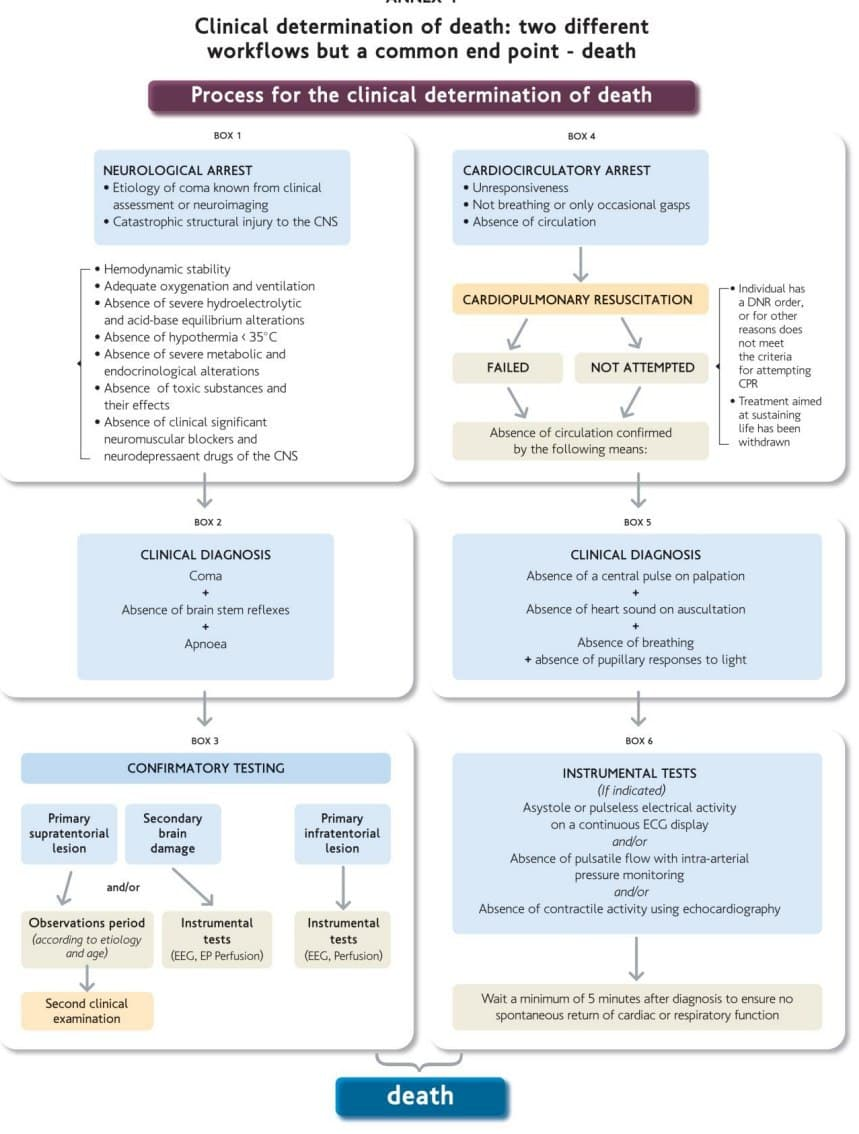
\includegraphics[width=11.93in]{Death} \end{center}

\hypertarget{persiapan-pemeriksaan-penunjang}{%
\section{Persiapan Pemeriksaan Penunjang}\label{persiapan-pemeriksaan-penunjang}}

\hypertarget{radiologi}{%
\subsection{Radiologi}\label{radiologi}}

\hypertarget{usg-abdomen-atas-bawah}{%
\subsubsection{USG Abdomen Atas Bawah}\label{usg-abdomen-atas-bawah}}

\hypertarget{usg-urologi}{%
\subsubsection{USG Urologi}\label{usg-urologi}}

\hypertarget{ct-stonografi}{%
\subsubsection{CT Stonografi}\label{ct-stonografi}}

\hypertarget{laboratorium}{%
\subsection{Laboratorium}\label{laboratorium}}

\hypertarget{asam-urat}{%
\subsubsection{Asam Urat}\label{asam-urat}}

\hypertarget{lipid-profil}{%
\subsubsection{Lipid Profil}\label{lipid-profil}}

\begin{center}\rule{0.5\linewidth}{0.5pt}\end{center}

\hypertarget{informasi-obat-esensial-ugd}{%
\chapter{Informasi Obat Esensial UGD}\label{informasi-obat-esensial-ugd}}

Pada bagian ini akan diisi dengan obat-obat rutin yang sering digunakan dalam penanganan pasien di UGD dikelompokkan berdasarkan kasus. Dosis obat dibuat berdasarkan pengalaman penyusun atas dasar pengetahuan dan instruksi dokter spesialis.

\hypertarget{general-1}{%
\section{General}\label{general-1}}

\hypertarget{sistem-perhitungan-obat-parenteral}{%
\subsection{Sistem Perhitungan Obat Parenteral}\label{sistem-perhitungan-obat-parenteral}}

Rumur Perhitungan Laju Syringe Pump

\textbf{Rumus 1}

\begin{equation}
\\
\frac{Dosis \times BB \times 60}{konsentrasi (mikrogram/cc)}
\\
\end{equation}

\textbf{Rumus 2}

\begin{equation}
\\
\frac{Dosis \times BB \times 60 \times Pengenceran(50 cc)}{Jumlah_obat (mcg)}
\end{equation}

Contoh Kasus:

\begin{itemize}
\tightlist
\item
  Obat untuk pasien berat badan 50 kg
\item
  Dosis awal titrasi vascon 0,1 mcg/kgBB/menit.
\item
  Sedaan Vascon 4 mg per vial.
\end{itemize}

\begin{equation}
\frac{0,1 mcg/kg/min \times 50 kg \times 60}{4000 mcg/50cc}
\end{equation}
\begin{equation}
\frac{5 mcg/min \times 60}{80mcg/cc}
\end{equation}
\begin{equation}
\frac{300 mcg/jam}{80 mcg/cc}
\end{equation}
\begin{equation}
\ 3,75 cc/jam
\end{equation}

\begin{center}\rule{0.5\linewidth}{0.5pt}\end{center}

\hypertarget{penyakit-dalam-2}{%
\section{Penyakit Dalam}\label{penyakit-dalam-2}}

\hypertarget{parenteral}{%
\subsection{Parenteral}\label{parenteral}}

\hypertarget{transfusi-darah}{%
\subsubsection{Transfusi Darah}\label{transfusi-darah}}

\hypertarget{wb}{%
\paragraph{WB}\label{wb}}

\hypertarget{prc}{%
\paragraph{PRC}\label{prc}}

\hypertarget{ffp}{%
\paragraph{FFP}\label{ffp}}

\hypertarget{tc}{%
\paragraph{TC}\label{tc}}

\hypertarget{albumin}{%
\subsubsection{Albumin}\label{albumin}}

\hypertarget{deksametason}{%
\subsubsection{Deksametason}\label{deksametason}}

\hypertarget{insulin}{%
\subsubsection{Insulin}\label{insulin}}

Sediaan:
* Rapid Acting (cnth: Novorapid): Flexpen isi 3 ml, tiap ml isi 100 unit (Total 300 Unit).
* Short Acting
* Intermediate Acting
* Long Acting

\hypertarget{drip-kad-hhs}{%
\paragraph{DRIP KAD HHS}\label{drip-kad-hhs}}

\hypertarget{regulasi-preoperasi}{%
\paragraph{Regulasi Preoperasi}\label{regulasi-preoperasi}}

\hypertarget{hiperkalemia}{%
\paragraph{Hiperkalemia}\label{hiperkalemia}}

\hypertarget{dosis-maintenance}{%
\paragraph{Dosis Maintenance}\label{dosis-maintenance}}

\hypertarget{kcl}{%
\subsubsection{KCL}\label{kcl}}

\hypertarget{natrium-bikarbonat}{%
\subsubsection{Natrium Bikarbonat}\label{natrium-bikarbonat}}

\hypertarget{oral}{%
\subsection{Oral}\label{oral}}

\begin{center}\rule{0.5\linewidth}{0.5pt}\end{center}

\hypertarget{paru-1}{%
\section{Paru}\label{paru-1}}

\hypertarget{parenteral-1}{%
\subsection{Parenteral}\label{parenteral-1}}

\hypertarget{aminofilin}{%
\subsubsection{Aminofilin}\label{aminofilin}}

\hypertarget{oral-1}{%
\subsection{Oral}\label{oral-1}}

\begin{center}\rule{0.5\linewidth}{0.5pt}\end{center}

\hypertarget{pediatri-2}{%
\section{Pediatri}\label{pediatri-2}}

\hypertarget{tablet}{%
\section{Tablet}\label{tablet}}

\hypertarget{sirup}{%
\section{Sirup}\label{sirup}}

\hypertarget{tetes}{%
\section{Tetes}\label{tetes}}

\hypertarget{nebul}{%
\section{Nebul}\label{nebul}}

\begin{itemize}
\tightlist
\item
  Lasalcom Inhaler Nebul respul 2.5 mg/2.5 ml (Ipratropium bromid 0,5 mg + Salbutamol 2,5 mg)
\end{itemize}

\hypertarget{parenteral-2}{%
\section{Parenteral}\label{parenteral-2}}

\hypertarget{antibiotik}{%
\subsection{Antibiotik}\label{antibiotik}}

\begin{itemize}
\tightlist
\item
  Cefotaxim 50 mg/kgBB/kali tiap 8-12 jam
\item
  Ceftriaxon 50 mg/kgBB/kali tiap 12 jam
  \_\_\_
\end{itemize}

\hypertarget{kardiovaskular-3}{%
\section{Kardiovaskular}\label{kardiovaskular-3}}

\hypertarget{parenteral-3}{%
\subsection{Parenteral}\label{parenteral-3}}

\hypertarget{dopamin}{%
\subsubsection{Dopamin}\label{dopamin}}

\begin{itemize}
\tightlist
\item
  sediaan 1 ampul = 200 mg
\end{itemize}

\begin{longtable}[]{@{}
  >{\raggedright\arraybackslash}p{(\columnwidth - 4\tabcolsep) * \real{0.34}}
  >{\raggedright\arraybackslash}p{(\columnwidth - 4\tabcolsep) * \real{0.24}}
  >{\raggedright\arraybackslash}p{(\columnwidth - 4\tabcolsep) * \real{0.41}}@{}}
\toprule
\begin{minipage}[b]{\linewidth}\raggedright
Kategori
\end{minipage} & \begin{minipage}[b]{\linewidth}\raggedright
Dosis
\end{minipage} & \begin{minipage}[b]{\linewidth}\raggedright
Keterangan
\end{minipage} \\
\midrule
\endhead
Rendah & 1-5 mcg/kgBB/menit & Reseptor dopaminergik terutama di ginjal, mesenterium dan pembuluh koroner \\
Sedang & 5-10 mcg/kgBB/Menit & Meningkatnya tekanan sistolik dan tekanan nadi tanpa mengubah tekanan diastolik \\
Tinggi & 10 - 20 mcg/kgBB/menit & Vasopressor \\
\bottomrule
\end{longtable}

Kontraindikasi:

\begin{itemize}
\tightlist
\item
  Hipovolemik belum terkoreksi
\item
  Takiartimia/fibrilasi ventrikel
\item
  Hipertiroid
\end{itemize}

\hypertarget{dobutamin}{%
\subsubsection{Dobutamin}\label{dobutamin}}

Beta 1 dan Beta 2 agonist, cardioselective, inotropic tanpa peningkatan HR signifikan (5-15x/min).

Kontrainfikasi pada pasien dengan hipertropik kardiomiopati

\begin{itemize}
\tightlist
\item
  Sediaan ampul = 250 mg
\end{itemize}

\begin{longtable}[]{@{}lll@{}}
\toprule
kategori & Dosis & Keterangan \\
\midrule
\endhead
rendah & 2-5 mcg/kgBB/menit & \\
Sedang & 5-10 mcg/kgBB/Menit & \\
Tinggi & 10-20 mcg/kgBB/menit & \\
\bottomrule
\end{longtable}

Kontraindikasi:

\begin{itemize}
\tightlist
\item
  Stenosis subaortik
\item
  Hipertropik Idiopatik
\end{itemize}

\hypertarget{norepinefrinvascon}{%
\subsubsection{Norepinefrin/Vascon}\label{norepinefrinvascon}}

Sediaan 1 ampul = 4 mg

\begin{longtable}[]{@{}lll@{}}
\toprule
Kategori & Dosis & Keterangan \\
\midrule
\endhead
& 0,1 - 0,5 mcg/kgBB/menit atau 5 - 30 mcg/min & \\
\bottomrule
\end{longtable}

\hypertarget{epinefrine}{%
\subsubsection{Epinefrine}\label{epinefrine}}

\begin{itemize}
\item
  Sediaan 1 ampul = 1 mg/ml (1:1000)
\item
  Dosis Awal: 1 -2 mcg/min (0,02 mcg/kg/min)
\item
  Dosis dinaikan 1 -2 mcg/min sesuai target
\end{itemize}

\hypertarget{nicardipin}{%
\subsubsection{Nicardipin}\label{nicardipin}}

\begin{itemize}
\tightlist
\item
  Sediaan: 10 mg/ampul
\item
  Dosis: 5 - 15 mg/jam
\end{itemize}

\hypertarget{isdn}{%
\subsubsection{ISDN}\label{isdn}}

\begin{itemize}
\tightlist
\item
  Sediaan: 1 ampul 10 mg
\item
  Dosis 1-10 mg/jam
\item
  Biasanya diencerkan 2 ampul
\end{itemize}

\hypertarget{nitrogliserin}{%
\subsubsection{Nitrogliserin}\label{nitrogliserin}}

\begin{itemize}
\tightlist
\item
  Sediaan = 50 mg (ampul)
\end{itemize}

\hypertarget{furosemid}{%
\subsubsection{Furosemid}\label{furosemid}}

\begin{itemize}
\tightlist
\item
  Sediaan = 20 mg/2cc (ampul)
\item
  Dosis initial: 5 - 10 mcg/min, bisa naik 5- 10 mcg/min setiap 5 menit
\item
  Dosis efektif 5 - 100 mcg/min
\end{itemize}

\hypertarget{heparin}{%
\subsubsection{Heparin}\label{heparin}}

\begin{itemize}
\tightlist
\item
  Sediaan : 25.000 Unit/vial
\item
  Obat dimasukan di 500 cc NS
\item
  Perhitungan kecepatan tetesan infus sesuai aturan tetes infus
\item
  Dosis:
\end{itemize}

\hypertarget{lmwh}{%
\subsubsection{LMWH}\label{lmwh}}

\hypertarget{digoxin}{%
\subsubsection{Digoxin}\label{digoxin}}

\hypertarget{adrenalinepinefrin}{%
\subsubsection{Adrenalin/Epinefrin}\label{adrenalinepinefrin}}

\hypertarget{sulfas-atropin}{%
\subsubsection{Sulfas Atropin}\label{sulfas-atropin}}

\hypertarget{amiodaron}{%
\subsubsection{Amiodaron}\label{amiodaron}}

\hypertarget{lidokain}{%
\subsubsection{Lidokain}\label{lidokain}}

\hypertarget{calcium-glukonas}{%
\subsubsection{Calcium Glukonas}\label{calcium-glukonas}}

\hypertarget{oral-nitrogliserin}{%
\subsection{Oral Nitrogliserin}\label{oral-nitrogliserin}}

\begin{center}\rule{0.5\linewidth}{0.5pt}\end{center}

\hypertarget{bedah-1}{%
\section{Bedah}\label{bedah-1}}

\begin{center}\rule{0.5\linewidth}{0.5pt}\end{center}

\hypertarget{anestesi-2}{%
\section{Anestesi}\label{anestesi-2}}

\hypertarget{analgetik}{%
\subsection{Analgetik}\label{analgetik}}

\hypertarget{morfin}{%
\subsubsection{Morfin}\label{morfin}}

\hypertarget{petidin}{%
\subsubsection{Petidin}\label{petidin}}

\hypertarget{fentanil-1}{%
\subsubsection{Fentanil}\label{fentanil-1}}

\hypertarget{ketorolac-1}{%
\subsubsection{Ketorolac}\label{ketorolac-1}}

\hypertarget{tramadol}{%
\subsubsection{Tramadol}\label{tramadol}}

\hypertarget{sedatif}{%
\subsection{Sedatif}\label{sedatif}}

\hypertarget{diazepam}{%
\subsubsection{Diazepam}\label{diazepam}}

\hypertarget{midazolam-1}{%
\subsubsection{Midazolam}\label{midazolam-1}}

\hypertarget{propofol-1}{%
\subsubsection{Propofol}\label{propofol-1}}

\hypertarget{muscle-relaxant}{%
\subsection{Muscle Relaxant}\label{muscle-relaxant}}

\begin{center}\rule{0.5\linewidth}{0.5pt}\end{center}

\hypertarget{neurologi-neurosurgery}{%
\section{Neurologi \& Neurosurgery}\label{neurologi-neurosurgery}}

\hypertarget{parenteral-4}{%
\subsection{Parenteral}\label{parenteral-4}}

\hypertarget{manitol}{%
\subsubsection{Manitol}\label{manitol}}

\hypertarget{nacl-3}\label{nacl-3}}

\hypertarget{fenitoin}{%
\subsubsection{Fenitoin}\label{fenitoin}}

\hypertarget{fenobarbital}{%
\subsubsection{Fenobarbital}\label{fenobarbital}}

\hypertarget{citicolin}{%
\subsubsection{Citicolin}\label{citicolin}}

\hypertarget{piracetam}{%
\subsubsection{Piracetam}\label{piracetam}}

\hypertarget{oral-2}{%
\subsection{Oral}\label{oral-2}}

\begin{center}\rule{0.5\linewidth}{0.5pt}\end{center}

\hypertarget{obstetri-gineklogi-2}{%
\section{Obstetri \& Gineklogi}\label{obstetri-gineklogi-2}}

\hypertarget{parenteral-5}{%
\subsection{Parenteral}\label{parenteral-5}}

\hypertarget{mgso4}{%
\subsubsection{MgSO4}\label{mgso4}}

\hypertarget{oral-3}{%
\subsection{Oral}\label{oral-3}}

\begin{center}\rule{0.5\linewidth}{0.5pt}\end{center}

\hypertarget{dermatologi-venereologi-1}{%
\section{Dermatologi \& Venereologi}\label{dermatologi-venereologi-1}}

\begin{center}\rule{0.5\linewidth}{0.5pt}\end{center}

\hypertarget{tht-1}{%
\section{THT}\label{tht-1}}

\begin{center}\rule{0.5\linewidth}{0.5pt}\end{center}

\hypertarget{mata-1}{%
\section{Mata}\label{mata-1}}

\begin{center}\rule{0.5\linewidth}{0.5pt}\end{center}

\hypertarget{hasil-rapat}{%
\chapter{Hasil Rapat}\label{hasil-rapat}}

\hypertarget{section}{%
\section{2021}\label{section}}

\begin{center}\rule{0.5\linewidth}{0.5pt}\end{center}

\hypertarget{september}{%
\subsection{September}\label{september}}

\begin{center}\rule{0.5\linewidth}{0.5pt}\end{center}

\hypertarget{oktober}{%
\subsection{Oktober}\label{oktober}}

\begin{center}\rule{0.5\linewidth}{0.5pt}\end{center}

\hypertarget{november}{%
\subsection{November}\label{november}}

Waktu: 26/11/2021

\begin{center}\rule{0.5\linewidth}{0.5pt}\end{center}

\hypertarget{desember}{%
\subsection{Desember}\label{desember}}

\begin{center}\rule{0.5\linewidth}{0.5pt}\end{center}

\hypertarget{section-1}{%
\section{2022}\label{section-1}}

\begin{center}\rule{0.5\linewidth}{0.5pt}\end{center}

\hypertarget{januari}{%
\subsection{Januari}\label{januari}}

\begin{center}\rule{0.5\linewidth}{0.5pt}\end{center}

\hypertarget{februari}{%
\subsection{Februari}\label{februari}}

\begin{center}\rule{0.5\linewidth}{0.5pt}\end{center}

\hypertarget{maret}{%
\subsection{Maret}\label{maret}}

\begin{center}\rule{0.5\linewidth}{0.5pt}\end{center}

\hypertarget{april}{%
\subsection{April}\label{april}}

\begin{center}\rule{0.5\linewidth}{0.5pt}\end{center}

\hypertarget{mei}{%
\subsection{Mei}\label{mei}}

\begin{center}\rule{0.5\linewidth}{0.5pt}\end{center}

\hypertarget{juni}{%
\subsection{Juni}\label{juni}}

\begin{center}\rule{0.5\linewidth}{0.5pt}\end{center}

\hypertarget{juli}{%
\subsection{Juli}\label{juli}}

\begin{center}\rule{0.5\linewidth}{0.5pt}\end{center}

\hypertarget{agustus}{%
\subsection{Agustus}\label{agustus}}

\begin{center}\rule{0.5\linewidth}{0.5pt}\end{center}

\hypertarget{refs}{}
\begin{CSLReferences}{1}{0}
\leavevmode\vadjust pre{\hypertarget{ref-R-rmarkdown}{}}%
Allaire, JJ, Yihui Xie, Jonathan McPherson, Javier Luraschi, Kevin Ushey, Aron Atkins, Hadley Wickham, Joe Cheng, Winston Chang, and Richard Iannone. \emph{Rmarkdown: Dynamic Documents for r}, 2021. \url{https://CRAN.R-project.org/package=rmarkdown}.

\leavevmode\vadjust pre{\hypertarget{ref-canonical_ubuntu_2021}{}}%
Canonical. {``Ubuntu {Server}.''} London, 2021. \url{https://wiki.ubuntu.com/FocalFossa/ReleaseNotes?_ga=2.202901329.1166669392.1642903327-1244252401.1642903327}.

\leavevmode\vadjust pre{\hypertarget{ref-R-base}{}}%
R Core Team. \emph{R: A Language and Environment for Statistical Computing}. Vienna, Austria: R Foundation for Statistical Computing, 2021. \url{https://www.R-project.org/}.

\leavevmode\vadjust pre{\hypertarget{ref-rstudio_team_rstudio_2021}{}}%
Rstudio. {``{RStudio}: {Integrated} {Development} for {R}.''} Boston: Rstudio PBC, 2021. \url{http://www.rstudio.com/}.

\leavevmode\vadjust pre{\hypertarget{ref-qrcode2021}{}}%
Teh, Victor, and Thierry Onkelinx. \emph{Qrcode: Generate QRcodes with r. Version 0.1.4}, 2021. \url{https://doi.org/10.5281/zenodo.5040088}.

\leavevmode\vadjust pre{\hypertarget{ref-R-bookdown}{}}%
Xie, Yihui. \emph{Bookdown: Authoring Books and Technical Documents with r Markdown}, 2021. \url{https://CRAN.R-project.org/package=bookdown}.

\leavevmode\vadjust pre{\hypertarget{ref-R-knitr}{}}%
---------. \emph{Knitr: A General-Purpose Package for Dynamic Report Generation in r}, 2021. \url{https://yihui.org/knitr/}.

\end{CSLReferences}

\end{document}
